\level{2}{Chuck}
	Dopo che in precedenza è stata fornita una descrizione generale di Chuck, è qui riportata la sua progettazione architetturale.\\
	La presente sezione riporta i risultati ottenuti tramite una rigida struttura:
	\begin{enumerate}
		\item vengono presentate e successivamente descritte le componenti individuate;
		\item vengono descritte le interazioni che possono avvenire tra le componenti che sono state individuate;
		\item vengono descritti e contestualizzati gli eventuali design pattern che sono stati utilizzati durante la progettazione delle componenti;
		\item vengono descritte le classi che sono state individuate all'interno di ciascuna componente (eventualmente suddivise per package di appartenenza);
		\item vengono descritte le interazioni tra le classi che sono state individuate;
		\item vengono descritti e contestualizzati i design pattern che sono stati utilizzati durante la progettazione delle classi.
	\end{enumerate}
	
	\level{3}{Descrizione delle componenti di Chuck}
		\begin{figure}[H]\centering
	        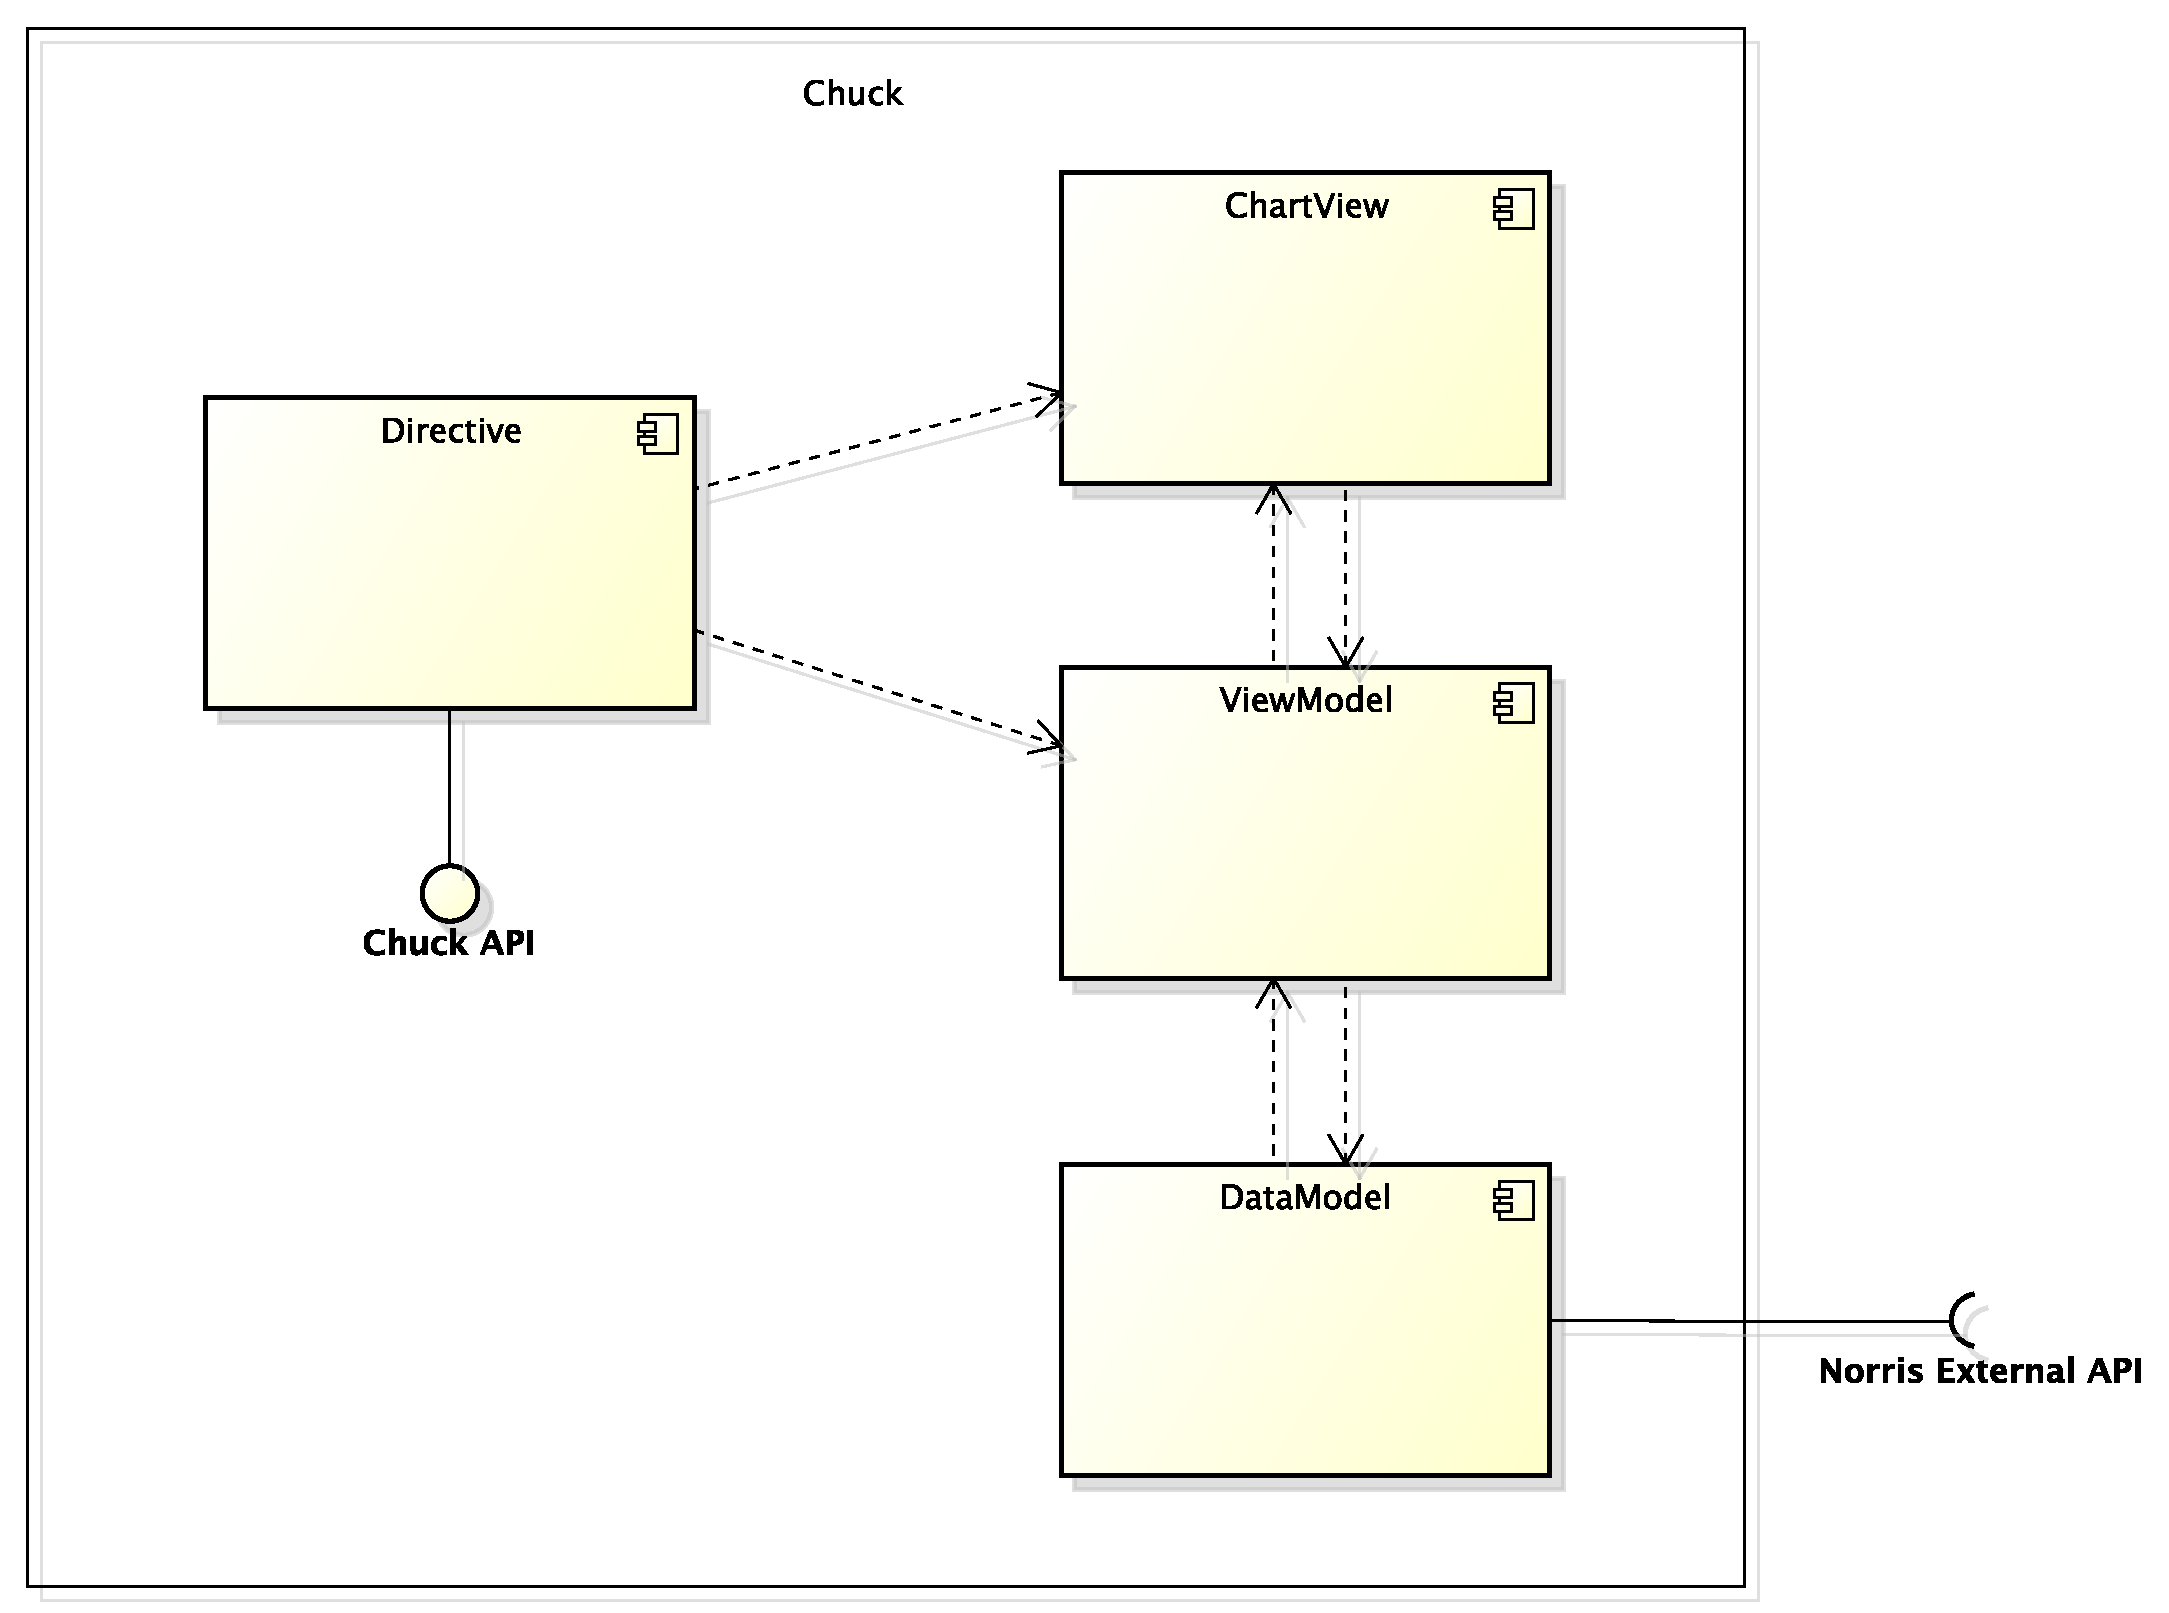
\includegraphics[width=\textwidth]{SpecificaTecnica/Pics/ComponentiChuck}
	        \caption{Diagramma delle componenti di Chuck}
	    \end{figure}
	    Di seguito vengono descritti i ruoli e le responsabilità delle varie componenti che sono state individuate durante la progettazione architetturale di Chuck.
    	\level{4}{Model}
			La componente Model è un modello che astrae i grafici visualizzati nella pagina web. Si divide a sua volta in due sottocomponenti:
			\begin{itemize}
				\item NorrisChart: contiene i dati riguardanti i grafici, assieme alle relative impostazioni. In particolare sono presenti i modelli di tutte le tipologie di chart implementati da Norris, ovvero Bar Chart, Line Chart, Map Chart e Table. Per ciascuna tipologia di grafico sono forniti i metodi per inserire i dati e configurare alcune impostazioni. Fornisce inoltre dei metodi per ottenere i valori di queste ultime, in modo da poterle riutilizzare per un altro grafico. Infine, per ogni grafico sono disponibili le stesse modalità di aggiornamento fornite da Norris.
				\item Services: si occupa della comunicazione con Norris attraverso l'utilizzo delle API esterne. In particolare gestisce le richieste dei grafici che lo sviluppatore client vuole inserire nel proprio sito e la ricezione degli aggiornamenti dei grafici stessi. Gestisce inoltre l'autenticazione presso l'istanza di Norris contenente tali grafici, fornendo allo sviluppatore le funzioni di login e logout.
			\end{itemize}

		\level{4}{Directive}
			La componente Directive fornisce le principali API di Chuck allo sviluppatore client. Le funzionalità offerte sono le seguenti:
			\begin{itemize}
				\item inserire nuovi grafici in un sito web;
				\item scegliere i grafici da inserire;
				\item scegliere il tag HTML in cui inserire un grafico;
				\item modificare alcune impostazioni dei grafici.
			\end{itemize}
			Questa componente comunica le sccelte dell'utente al ViewModel e alla View.
    		
		\level{4}{View}
			La componente View ha il compito di visualizzare i grafici all'interno della pagina web. I grafici possono essere del tipo Bar Chart, Line Chart, Map Chart e Table. Quando un grafico viene aggiornato, questa componente si occupa di aggiornare anche la sua visualizzazione nella pagina web. Un altro compito della View consiste nell'accogliere gli input inerenti il filtraggio dei dati di un determinato chart e inviarli al ViewModel.
			
		\level{4}{View Model}
			La componente ViewModel fa da tramite tra la View e il Model. Si occupa di richiamare le funzionalità delle librerie grafiche che permettono alla View di visualizzare i grafici. Inoltre ha lo scopo di ricevere gli input provenienti dalla View ed effettuarne la gestione. L'input consiste in un sottoinsieme di dataset scelti dall'utente che sta visualizzando la pagina web. Il ViewModel deve far sì che vengano visualizzati solo questi dataset, in modo da permettere all'utente di applicare un filtro sulle serie.
			    
	\level{3}{Descrizione delle interazioni tra le componenti}
		\level{4}{Model - ViewModel}
			Quando avviene una modifica nel Model, una notifica avvisa il ViewModel dell'avvenuto cambiamento. In particolare quando arriva l'aggiormento di un grafico già presente, dopo aver aggiornato i dati del grafico il Model manda una notifica al ViewModel.

		\level{4}{ViewModel - Model}
			Quando il ViewModel deve aggiornare la visualizzazione del grafico, esso effettua una query sul Model per ottenere le nuove informazioni relative al grafico da aggiornare. Ciò avviene dopo che il ViewModel è stato notificato riguardo un cambiamento avvenuto nel Model. 
			
		\level{4}{View - ViewModel}
			Quando la View riceve un input dall'utente, una notifica avvisa il ViewModel in modo che intraprenda l'azione per gestirla. In particolare la View notifica il ViewModel quando l'utente seleziona i dataset che vuole visualizzare. La View invia al ViewModel anche le informazioni relative ai dataset selezionati, in modo che quets'ultimo possa effettuare le operazioni di filtraggio dei dati.
			
		\level{4}{ViewModel - View}
			Il ViewModel si occupa di aggiornare la View quando i dati del Model vengono modificati. In particolare ciò avviene dopo l'inserimento di un nuovo grafico o dopo un aggiornamento. Inoltre il ViewModel si occupa di modificare la View in seguito ad una richiesta di filtraggio dei dati.
				
		\level{4}{Directive - ViewModel}
			La Directive demanda l'implementazione delle funzionalità fornite dalle API di Chuck ai metodi del ViewModel. Si occupa dunque di richiamare i metodi del ViewModel necessari, passando loro i parametri corretti.
			
		\level{4}{Directive - View}
			La Directive si occupa di selezionare la View corrispondente al tipo di grafico che si vuole inserire nella pagina web.
	\level{3}{Design pattern utilizzati con le componenti}
		Riportiamo di seguito i pattern architetturali utilizzati nella progettazione delle componenti di Chuck.
		\level{4}{Model View ViewModel}
			Model-View-ViewModel (MVVM) è un pattern architetturale utilizzato per separare il codice in blocchi di funzionalità ben distinte.\\
			Per la descrizione del pattern e dei vantaggi derivanti dalla sua applicazione si rimanda all'appendice \nameref{app:???}.
			\level{5}{Contesto di utilizzo}
				L'MVVM viene utilizzato per dividere le classi della libreria Chuck in tre grandi componenti:
				\begin{itemize}
					\item View;
					\item Model;
					\item ViewModel;
				\end{itemize}
	
	\level{3}{Descrizione delle classi di Chuck}
		In questa sezione sono presenti le descrizioni di tutte le classi presenti all'interno del \insglo{prodotto} \insglo{Chuck}. Queste sono state suddivise in base al componente nelle quali sono contenute.
		\level{1}{Chuck}
    \level{2}{Specifica dei componenti}
        Nella presente sezione è stata riportata e documentata la progettazione di dettaglio del \insglo{prodotto} \insglo{Chuck}. Si noti che tale progettazione deriva direttamente dalla progettazione architetturale che può essere trovata all'interno del documento \insdoc{Specifica Tecnica v5.00}. I risultati ottenuti sono stati organizzati e presentati secondo la seguente struttura:
        \begin{enumerate}
            \item vengono innanzitutto presentate le varie classi che sono state individuate. Per ognuna di esse si indica il nome, il tipo, l'eventuale astrattezza, la visibilità e il fatto che estenda altre classi oppure no. In aggiunta a ciò, viene presentata una descrizione completa del ruolo e delle responsabilità della classe oltre a una documentazione completa riguardante tutti gli attributi e i metodi presenti all'interno.
            \item in secondo luogo vengono presentati i diagrammi di sequenza, che hanno lo scopo di descrivere scenari (determinate sequenze di azioni in cui tutte le scelte sono già state effettuate). Essi vengono usati per descrivere le relazioni che intercorrono, in termini di messaggi, tra attori, oggetti ed entità del sistema \insglo{Chuck}.
        \end{enumerate}
        Le regole che sono state rispettate, gli strumenti che sono stati usati e le procedure che sono state effettuate possono essere trovate all'interno del documento \insdoc{Norme di Progetto v6.00}.
        \level{3}{Gerarchie presenti in Chuck}
            Di seguito vengono elencate tutte le gerarchie presenti in \insglo{Chuck} per fornire in forma visiva tutti i tipi implementati/estesi dalle singole componenti.
            \begin{itemize}
                \item Gerarchie in Model::NorrisChart \\
                    La seguente gerarchia rappresenta tutte le tipologie di chart utilizzate in \insglo{Chuck}.
                    \begin{figure}[H]
                        \centering
                        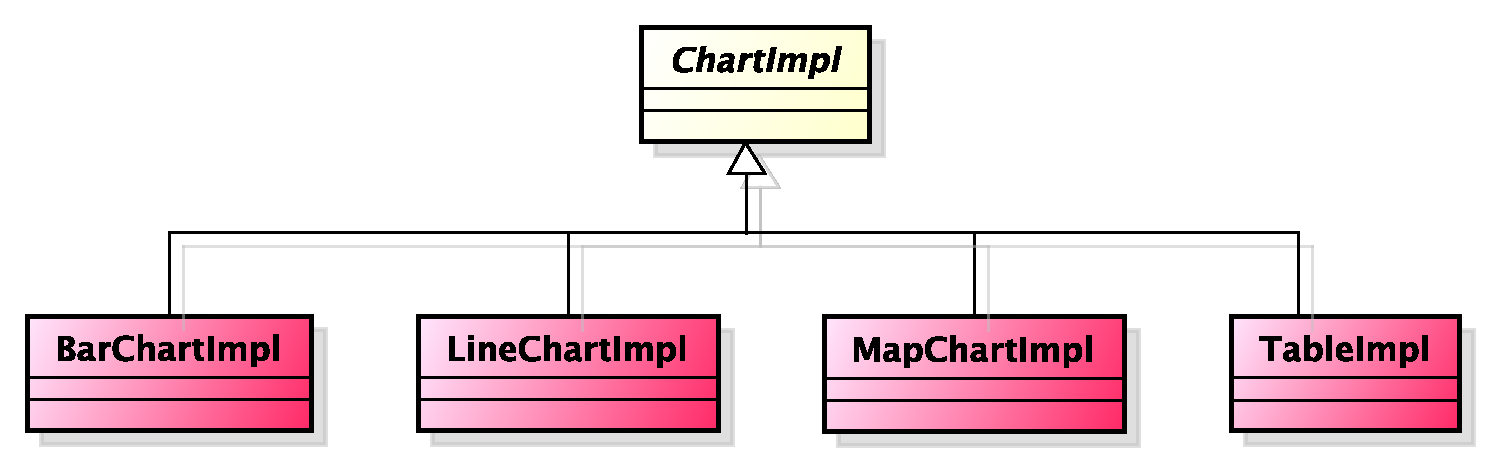
\includegraphics[width=1\textwidth]{DefinizioneDiProdotto/Pics/Gerarchie/ModelChartImpl.pdf}
                        \caption{Diagramma gerarchia ChartImpl in Chuck Model::NorrisChart }
                    \end{figure}
                    La seguente gerarchia rappresenta tutte le tipologie di chart factory che permettono la creazione dei vari chart.
                    \begin{figure}[H]
                        \centering
                        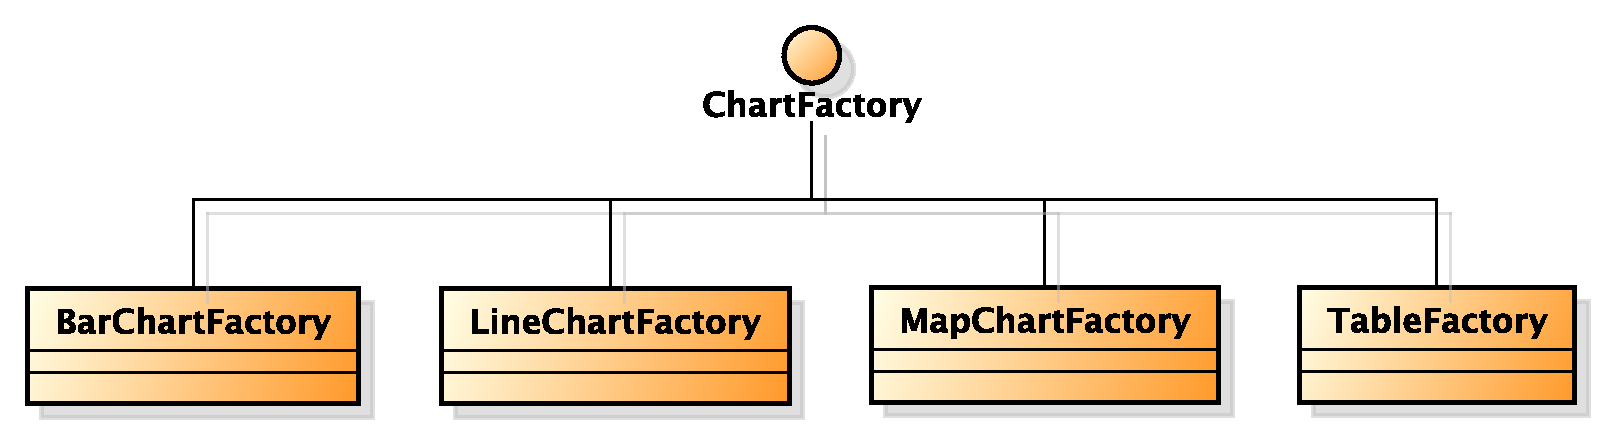
\includegraphics[width=1\textwidth]{DefinizioneDiProdotto/Pics/Gerarchie/ModelFactory.pdf}
                        \caption{Diagramma gerarchia ChartFactory in Chuck Model::NorrisChart}
                    \end{figure}
                    La seguente gerarchia rappresenta tutte le tipologie di updater che possono esser utilizzate per aggiornare un chart.
                    \begin{figure}[H]
                        \centering
                        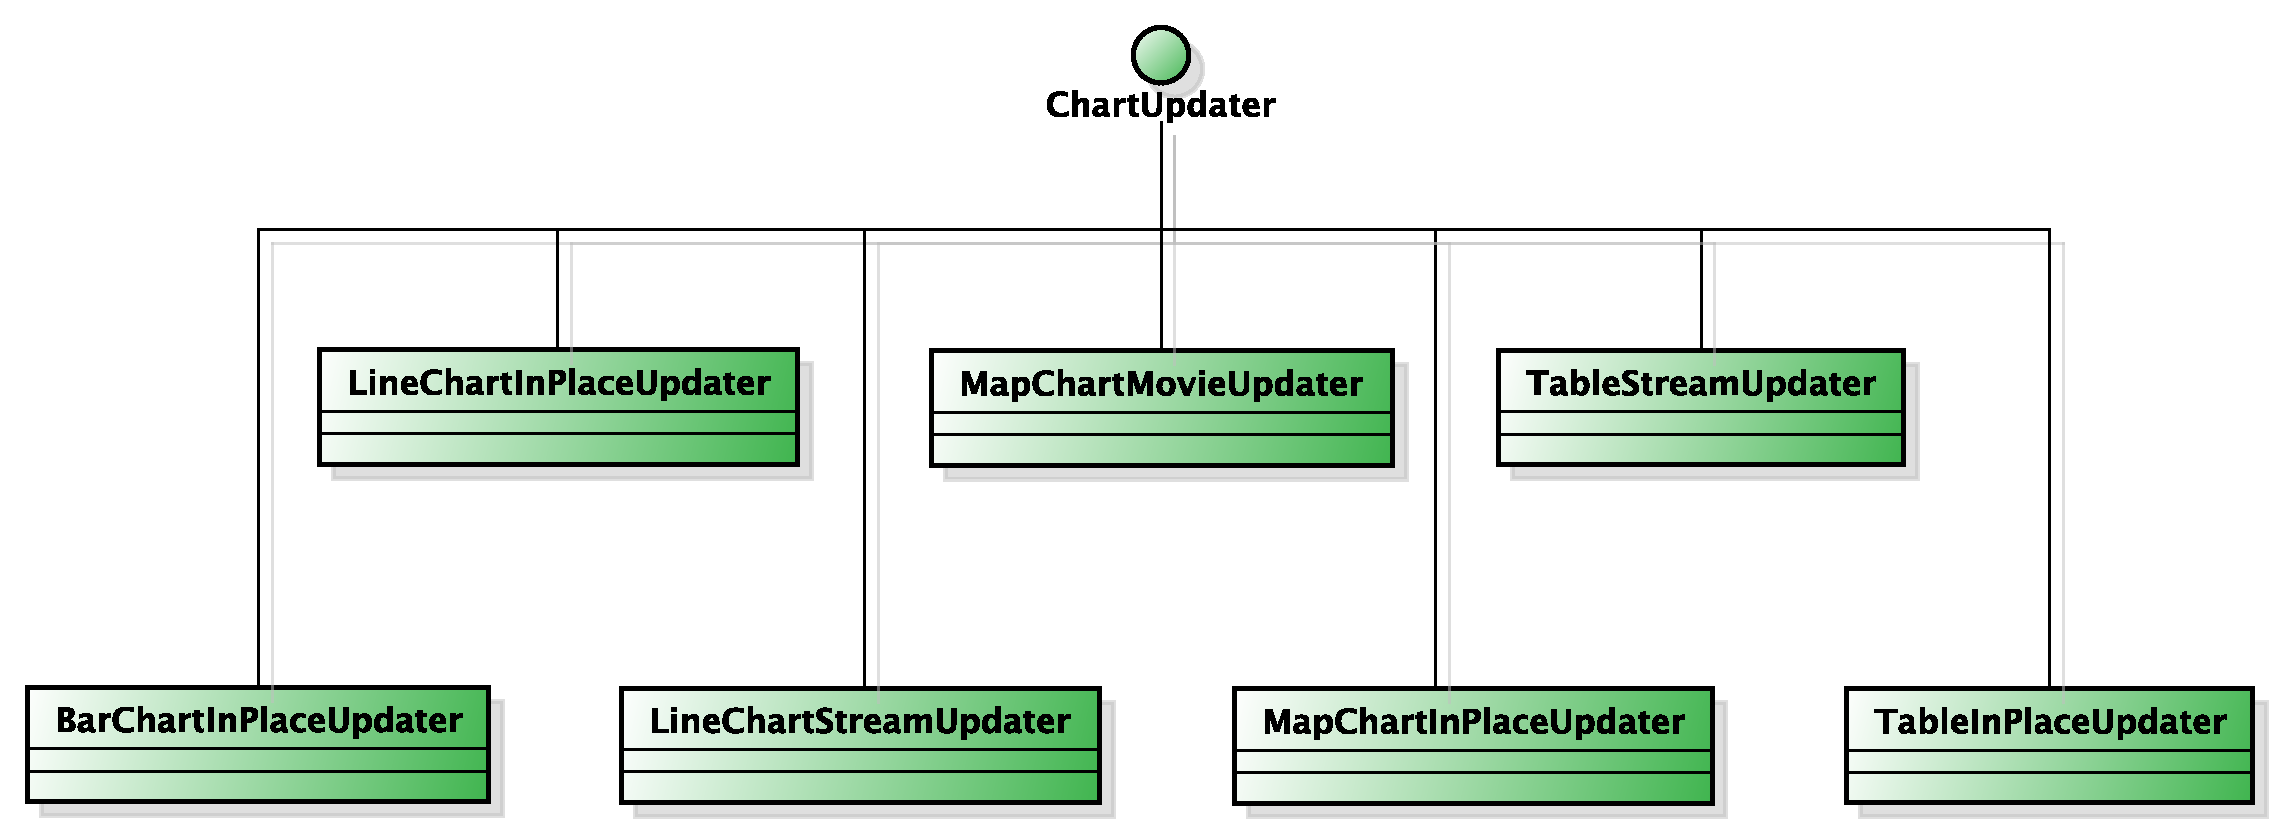
\includegraphics[width=1\textwidth]{DefinizioneDiProdotto/Pics/Gerarchie/ModelUpdater.pdf}
                        \caption{Diagramma gerarchia Updater in Chuck Model::NorrisChart }
                    \end{figure}
                \item Gerarchie in Model::Services \\
                    La seguente gerarchia rappresenta i servizi utilizzati in \insglo{Chuck}.
                    \begin{figure}[H]
                        \centering
                        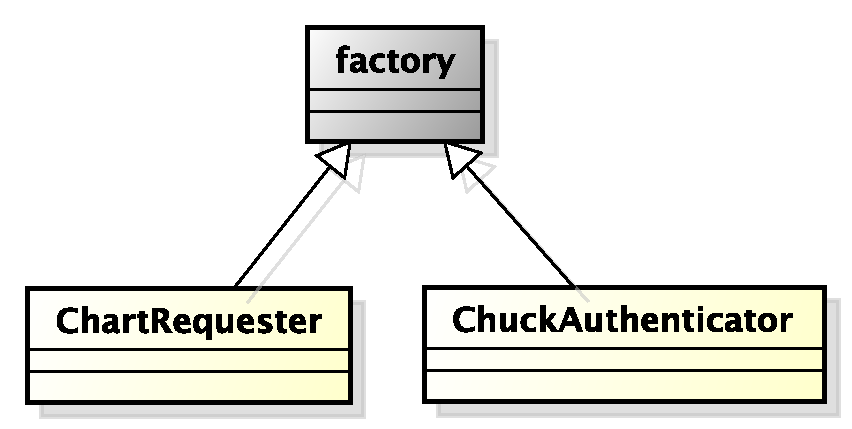
\includegraphics[width=1\textwidth]{DefinizioneDiProdotto/Pics/Gerarchie/ChuckService.pdf}
                        \caption{Diagramma gerarchia dei services in Chuck Model::Services}
                    \end{figure}
                \item Gerarchie in ViewModel \\
                    La seguente gerarchia rappresenta tutte le view-model utilizzate in \insglo{Chuck}.
                    \begin{figure}[H]
                        \centering
                        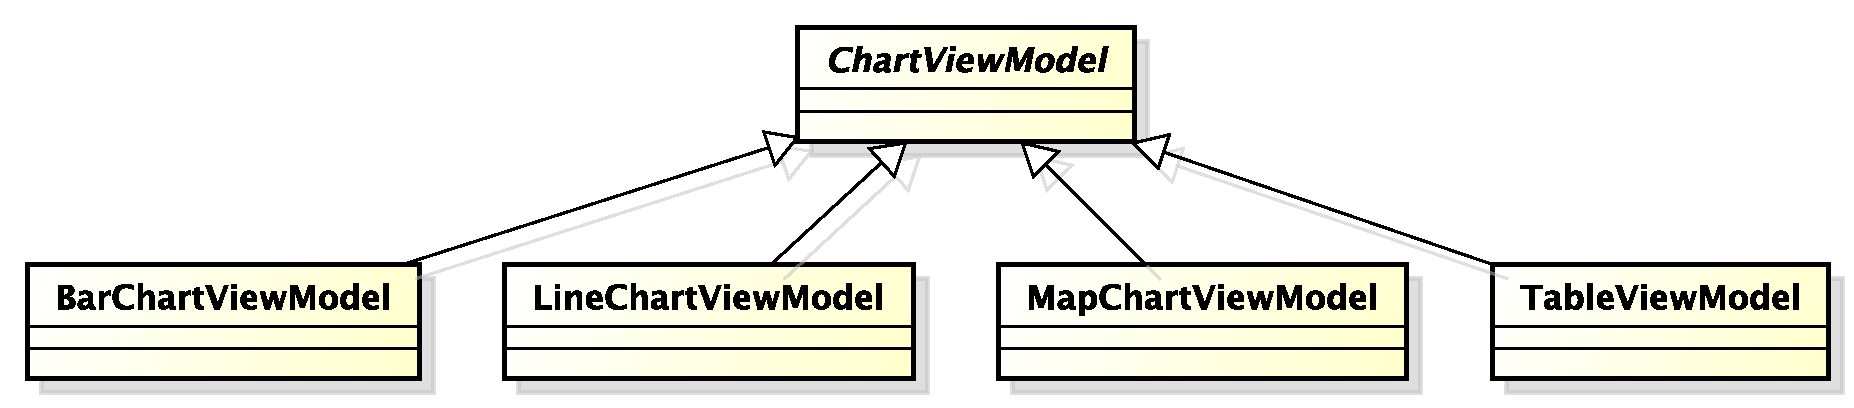
\includegraphics[width=1\textwidth]{DefinizioneDiProdotto/Pics/Gerarchie/ChuckViewModel.pdf}
                        \caption{Diagramma gerarchia dei view-model in Chuck ViewModel}
                    \end{figure}
                \item Gerarchie in Directive \\
                    La seguente gerarchia rappresenta le varie directive utilizzate in \insglo{Chuck}.
                    \begin{figure}[H]
                        \centering
                        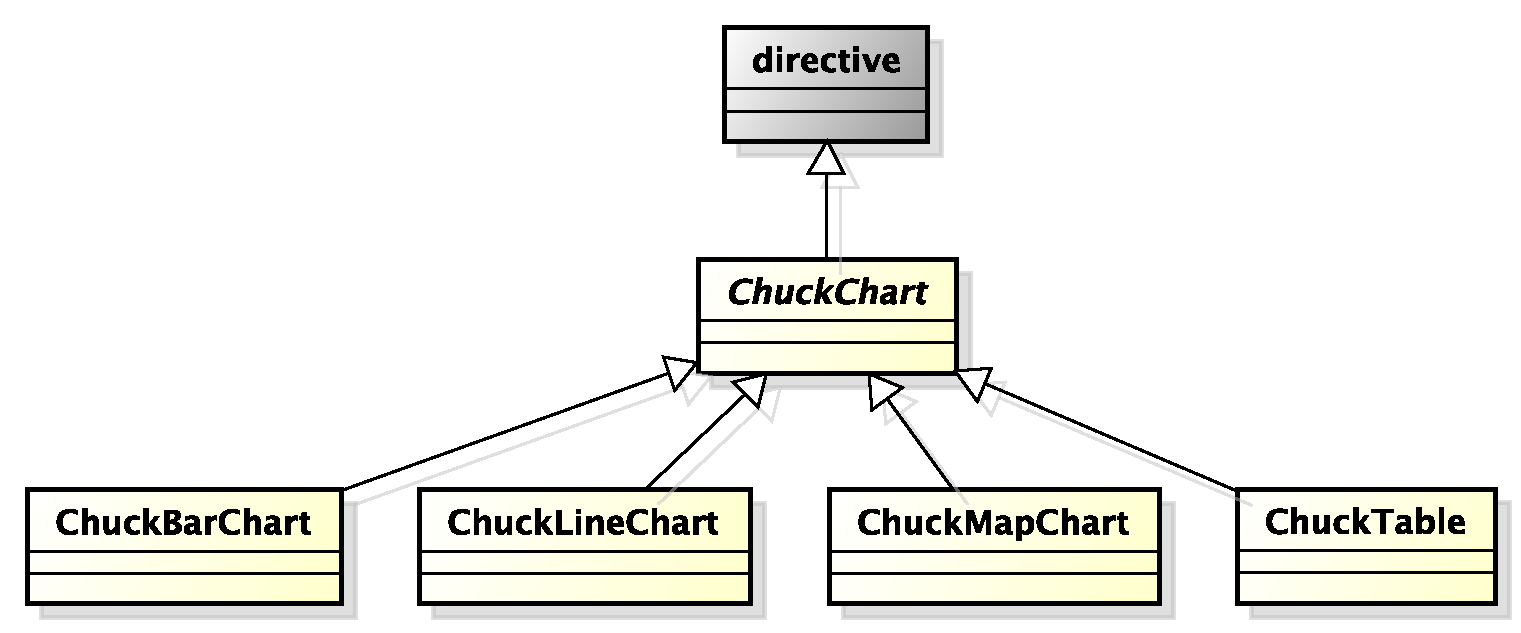
\includegraphics[width=1\textwidth]{DefinizioneDiProdotto/Pics/Gerarchie/ChuckDirective.pdf}
                        \caption{Diagramma gerarchia delle directive in Chuck Directive}
                    \end{figure}
                \item Gerarchie in View \\
                    La seguente gerarchia rappresenta le varie view utilizzate in \insglo{Chuck}.
                    \begin{figure}[H]
                        \centering
                        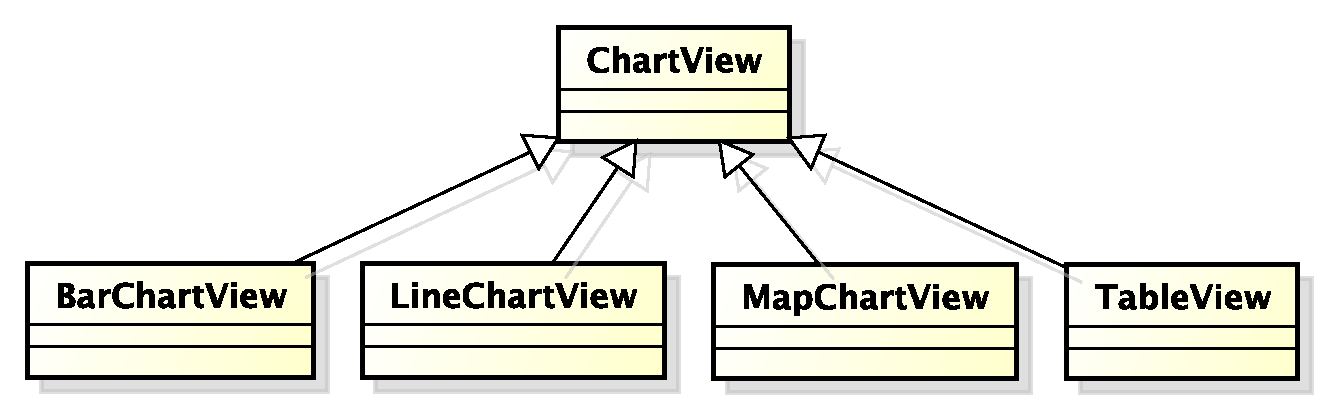
\includegraphics[width=1\textwidth]{DefinizioneDiProdotto/Pics/Gerarchie/ChuckView.pdf}
                        \caption{Diagramma gerarchia delle view in Chuck View}
                    \end{figure}
            \end{itemize}

        \level{3}{Classi}
            In tale sezione sono riportate delle descrizioni dettagliate delle classi individuate all'interno del documento \insdoc{Specifica Tecnica v4.00}. Tali classi sono presentate e organizzate in modo gerarchico, mantenendo una suddivisione per \insglo{package} di appartenenza.
            \level{1}{Chuck}
    \level{2}{Specifica dei componenti}
        Nella presente sezione è stata riportata e documentata la progettazione di dettaglio del \insglo{prodotto} \insglo{Chuck}. Si noti che tale progettazione deriva direttamente dalla progettazione architetturale che può essere trovata all'interno del documento \insdoc{Specifica Tecnica v5.00}. I risultati ottenuti sono stati organizzati e presentati secondo la seguente struttura:
        \begin{enumerate}
            \item vengono innanzitutto presentate le varie classi che sono state individuate. Per ognuna di esse si indica il nome, il tipo, l'eventuale astrattezza, la visibilità e il fatto che estenda altre classi oppure no. In aggiunta a ciò, viene presentata una descrizione completa del ruolo e delle responsabilità della classe oltre a una documentazione completa riguardante tutti gli attributi e i metodi presenti all'interno.
            \item in secondo luogo vengono presentati i diagrammi di sequenza, che hanno lo scopo di descrivere scenari (determinate sequenze di azioni in cui tutte le scelte sono già state effettuate). Essi vengono usati per descrivere le relazioni che intercorrono, in termini di messaggi, tra attori, oggetti ed entità del sistema \insglo{Chuck}.
        \end{enumerate}
        Le regole che sono state rispettate, gli strumenti che sono stati usati e le procedure che sono state effettuate possono essere trovate all'interno del documento \insdoc{Norme di Progetto v6.00}.
        \level{3}{Gerarchie presenti in Chuck}
            Di seguito vengono elencate tutte le gerarchie presenti in \insglo{Chuck} per fornire in forma visiva tutti i tipi implementati/estesi dalle singole componenti.
            \begin{itemize}
                \item Gerarchie in Model::NorrisChart \\
                    La seguente gerarchia rappresenta tutte le tipologie di chart utilizzate in \insglo{Chuck}.
                    \begin{figure}[H]
                        \centering
                        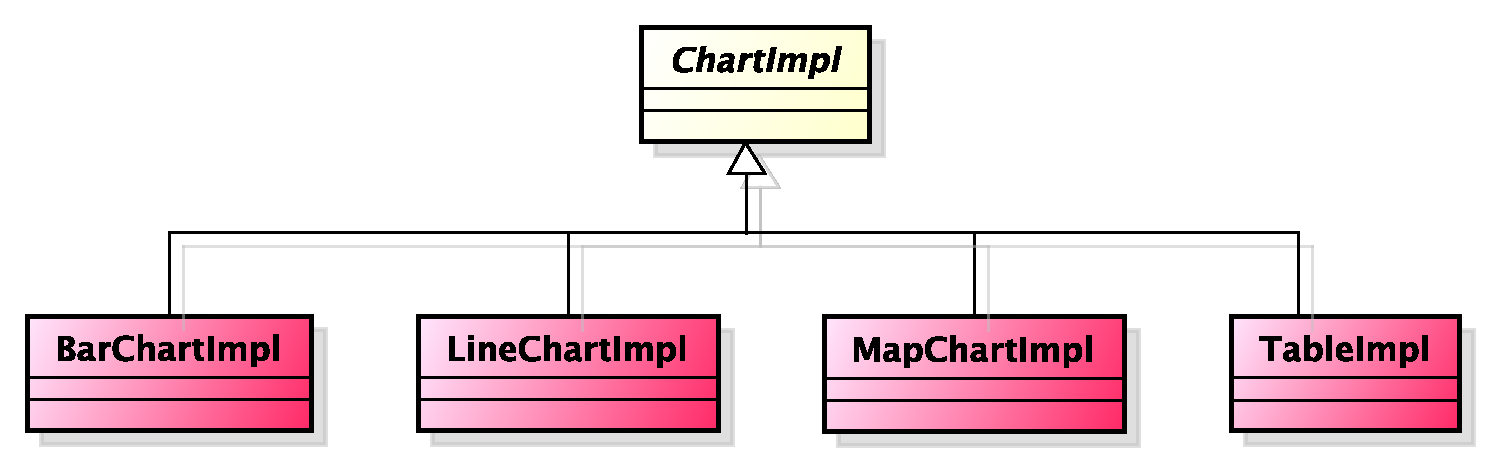
\includegraphics[width=1\textwidth]{DefinizioneDiProdotto/Pics/Gerarchie/ModelChartImpl.pdf}
                        \caption{Diagramma gerarchia ChartImpl in Chuck Model::NorrisChart }
                    \end{figure}
                    La seguente gerarchia rappresenta tutte le tipologie di chart factory che permettono la creazione dei vari chart.
                    \begin{figure}[H]
                        \centering
                        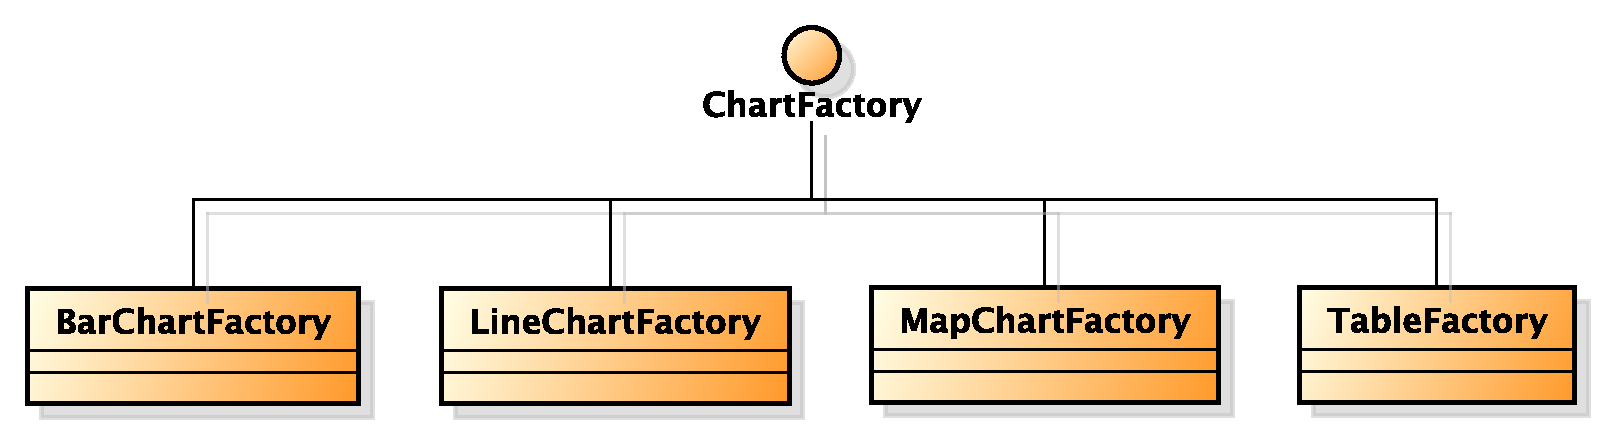
\includegraphics[width=1\textwidth]{DefinizioneDiProdotto/Pics/Gerarchie/ModelFactory.pdf}
                        \caption{Diagramma gerarchia ChartFactory in Chuck Model::NorrisChart}
                    \end{figure}
                    La seguente gerarchia rappresenta tutte le tipologie di updater che possono esser utilizzate per aggiornare un chart.
                    \begin{figure}[H]
                        \centering
                        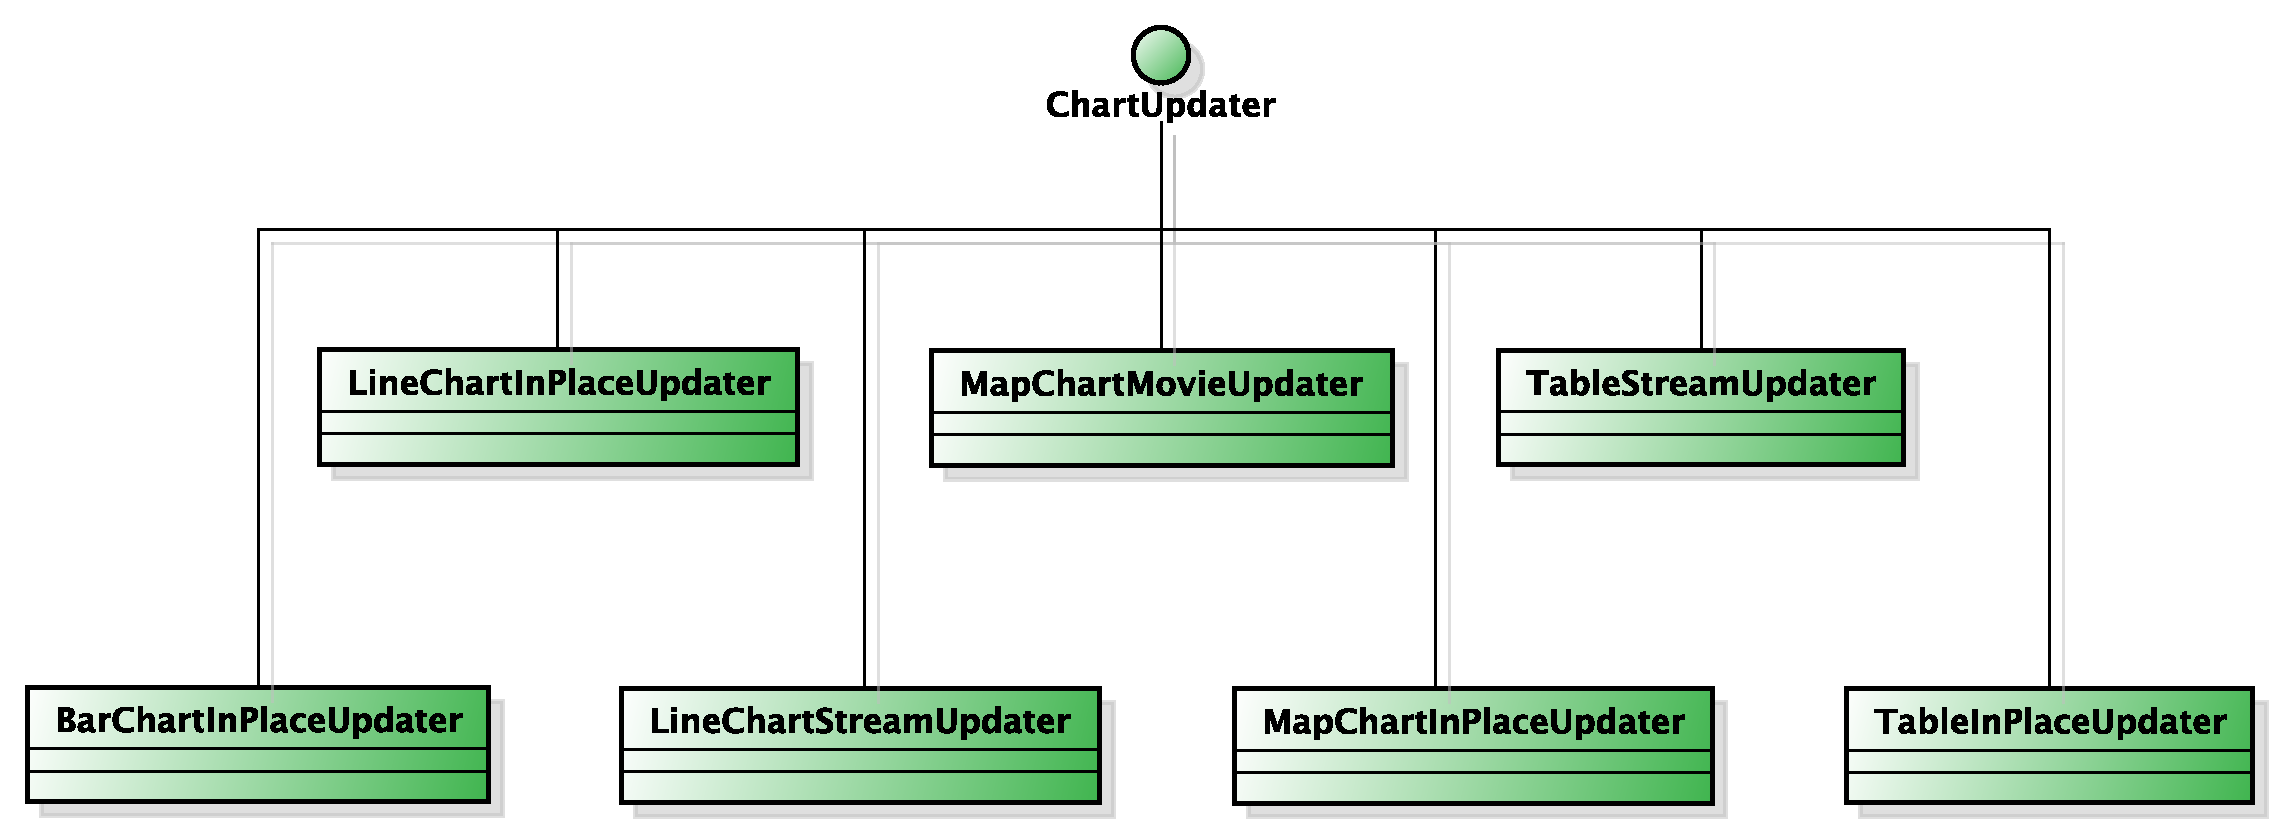
\includegraphics[width=1\textwidth]{DefinizioneDiProdotto/Pics/Gerarchie/ModelUpdater.pdf}
                        \caption{Diagramma gerarchia Updater in Chuck Model::NorrisChart }
                    \end{figure}
                \item Gerarchie in Model::Services \\
                    La seguente gerarchia rappresenta i servizi utilizzati in \insglo{Chuck}.
                    \begin{figure}[H]
                        \centering
                        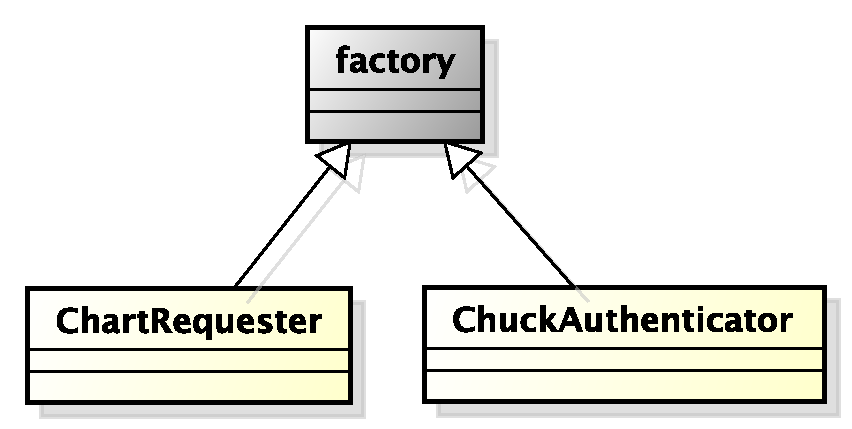
\includegraphics[width=1\textwidth]{DefinizioneDiProdotto/Pics/Gerarchie/ChuckService.pdf}
                        \caption{Diagramma gerarchia dei services in Chuck Model::Services}
                    \end{figure}
                \item Gerarchie in ViewModel \\
                    La seguente gerarchia rappresenta tutte le view-model utilizzate in \insglo{Chuck}.
                    \begin{figure}[H]
                        \centering
                        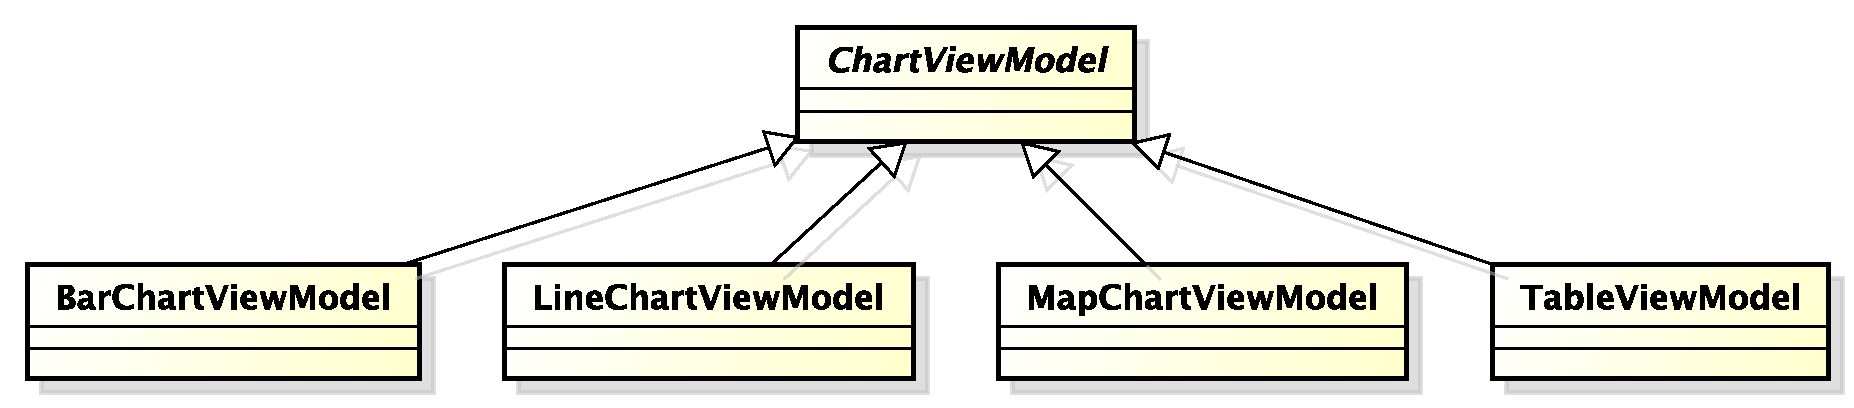
\includegraphics[width=1\textwidth]{DefinizioneDiProdotto/Pics/Gerarchie/ChuckViewModel.pdf}
                        \caption{Diagramma gerarchia dei view-model in Chuck ViewModel}
                    \end{figure}
                \item Gerarchie in Directive \\
                    La seguente gerarchia rappresenta le varie directive utilizzate in \insglo{Chuck}.
                    \begin{figure}[H]
                        \centering
                        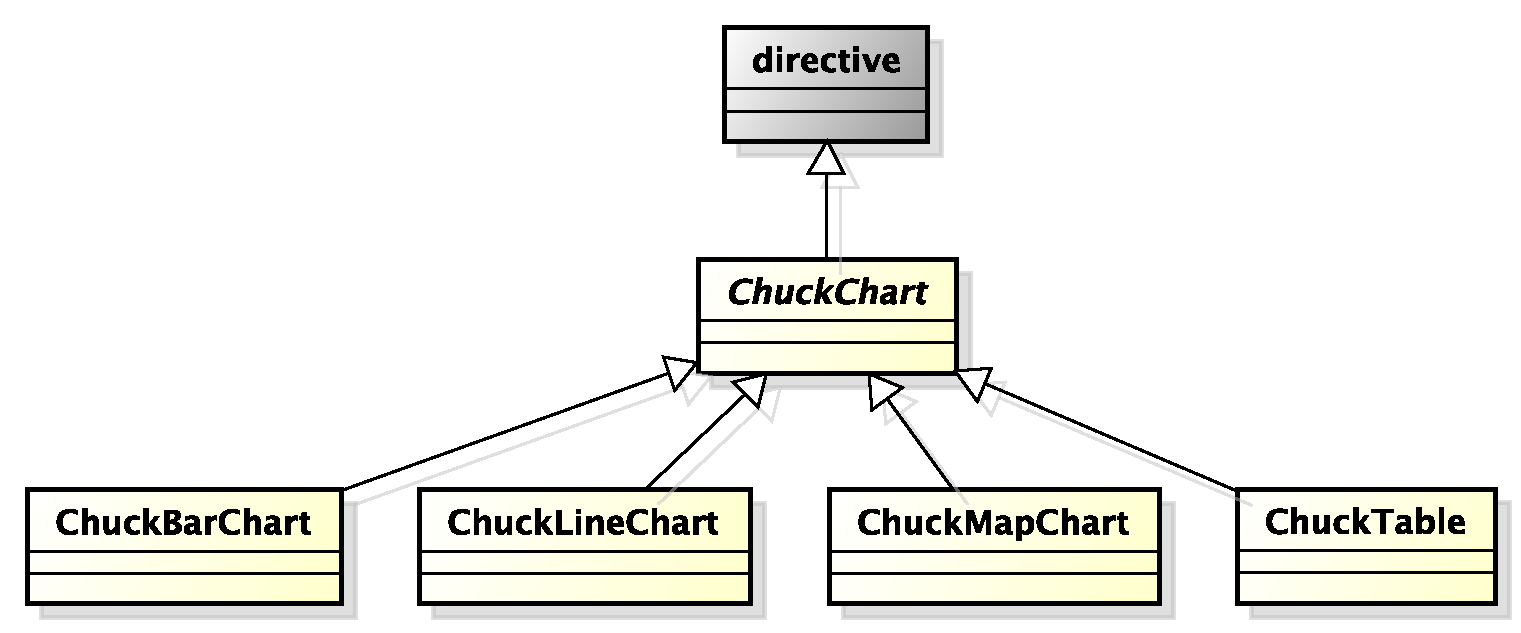
\includegraphics[width=1\textwidth]{DefinizioneDiProdotto/Pics/Gerarchie/ChuckDirective.pdf}
                        \caption{Diagramma gerarchia delle directive in Chuck Directive}
                    \end{figure}
                \item Gerarchie in View \\
                    La seguente gerarchia rappresenta le varie view utilizzate in \insglo{Chuck}.
                    \begin{figure}[H]
                        \centering
                        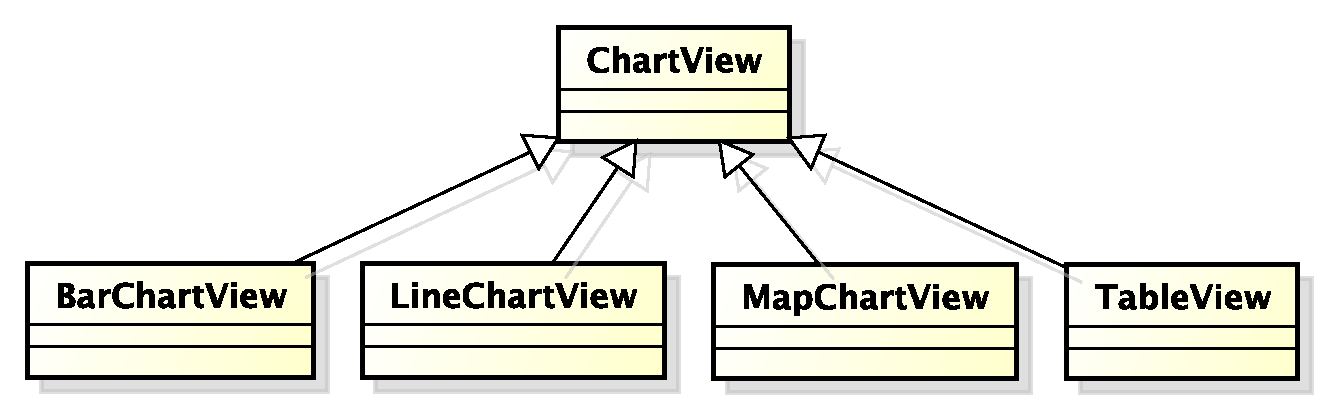
\includegraphics[width=1\textwidth]{DefinizioneDiProdotto/Pics/Gerarchie/ChuckView.pdf}
                        \caption{Diagramma gerarchia delle view in Chuck View}
                    \end{figure}
            \end{itemize}

        \level{3}{Classi}
            In tale sezione sono riportate delle descrizioni dettagliate delle classi individuate all'interno del documento \insdoc{Specifica Tecnica v4.00}. Tali classi sono presentate e organizzate in modo gerarchico, mantenendo una suddivisione per \insglo{package} di appartenenza.
            \level{1}{Chuck}
    \level{2}{Specifica dei componenti}
        Nella presente sezione è stata riportata e documentata la progettazione di dettaglio del \insglo{prodotto} \insglo{Chuck}. Si noti che tale progettazione deriva direttamente dalla progettazione architetturale che può essere trovata all'interno del documento \insdoc{Specifica Tecnica v5.00}. I risultati ottenuti sono stati organizzati e presentati secondo la seguente struttura:
        \begin{enumerate}
            \item vengono innanzitutto presentate le varie classi che sono state individuate. Per ognuna di esse si indica il nome, il tipo, l'eventuale astrattezza, la visibilità e il fatto che estenda altre classi oppure no. In aggiunta a ciò, viene presentata una descrizione completa del ruolo e delle responsabilità della classe oltre a una documentazione completa riguardante tutti gli attributi e i metodi presenti all'interno.
            \item in secondo luogo vengono presentati i diagrammi di sequenza, che hanno lo scopo di descrivere scenari (determinate sequenze di azioni in cui tutte le scelte sono già state effettuate). Essi vengono usati per descrivere le relazioni che intercorrono, in termini di messaggi, tra attori, oggetti ed entità del sistema \insglo{Chuck}.
        \end{enumerate}
        Le regole che sono state rispettate, gli strumenti che sono stati usati e le procedure che sono state effettuate possono essere trovate all'interno del documento \insdoc{Norme di Progetto v6.00}.
        \level{3}{Gerarchie presenti in Chuck}
            Di seguito vengono elencate tutte le gerarchie presenti in \insglo{Chuck} per fornire in forma visiva tutti i tipi implementati/estesi dalle singole componenti.
            \begin{itemize}
                \item Gerarchie in Model::NorrisChart \\
                    La seguente gerarchia rappresenta tutte le tipologie di chart utilizzate in \insglo{Chuck}.
                    \begin{figure}[H]
                        \centering
                        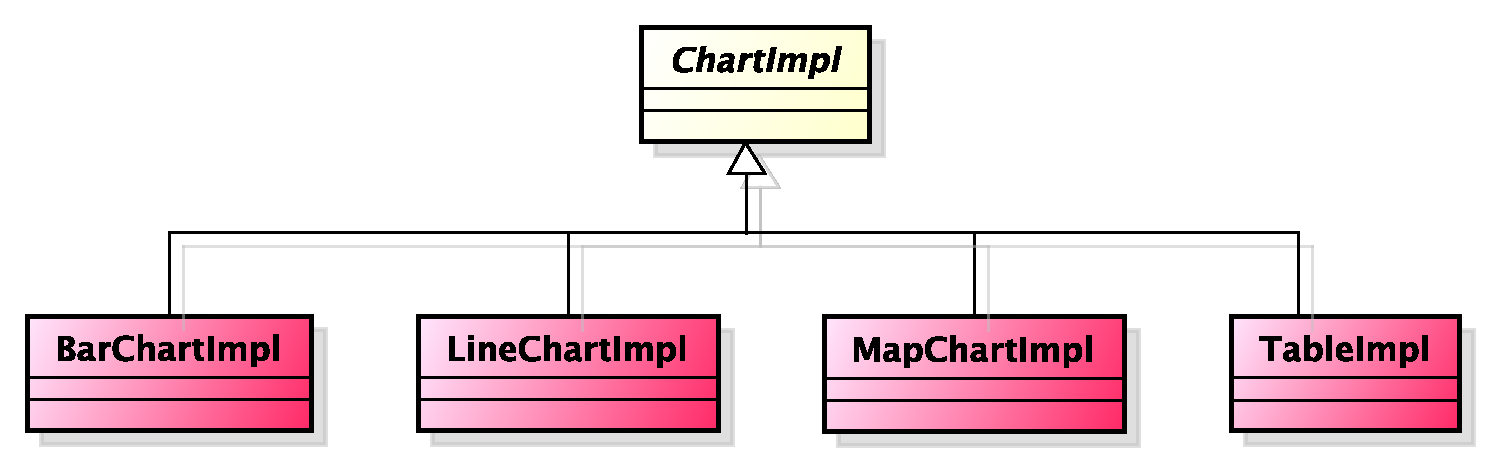
\includegraphics[width=1\textwidth]{DefinizioneDiProdotto/Pics/Gerarchie/ModelChartImpl.pdf}
                        \caption{Diagramma gerarchia ChartImpl in Chuck Model::NorrisChart }
                    \end{figure}
                    La seguente gerarchia rappresenta tutte le tipologie di chart factory che permettono la creazione dei vari chart.
                    \begin{figure}[H]
                        \centering
                        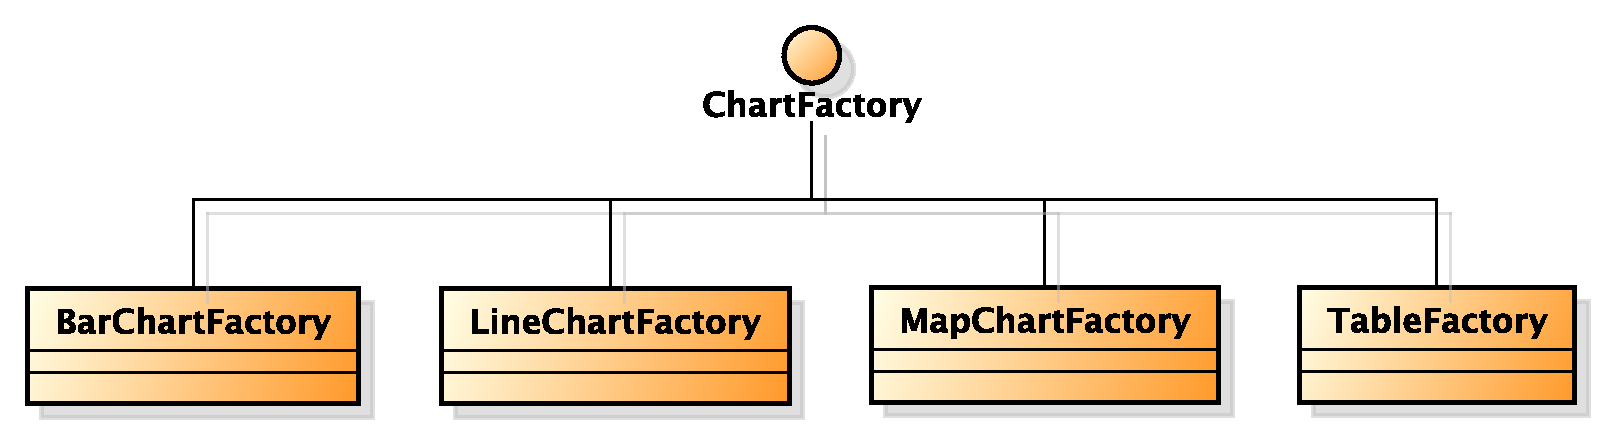
\includegraphics[width=1\textwidth]{DefinizioneDiProdotto/Pics/Gerarchie/ModelFactory.pdf}
                        \caption{Diagramma gerarchia ChartFactory in Chuck Model::NorrisChart}
                    \end{figure}
                    La seguente gerarchia rappresenta tutte le tipologie di updater che possono esser utilizzate per aggiornare un chart.
                    \begin{figure}[H]
                        \centering
                        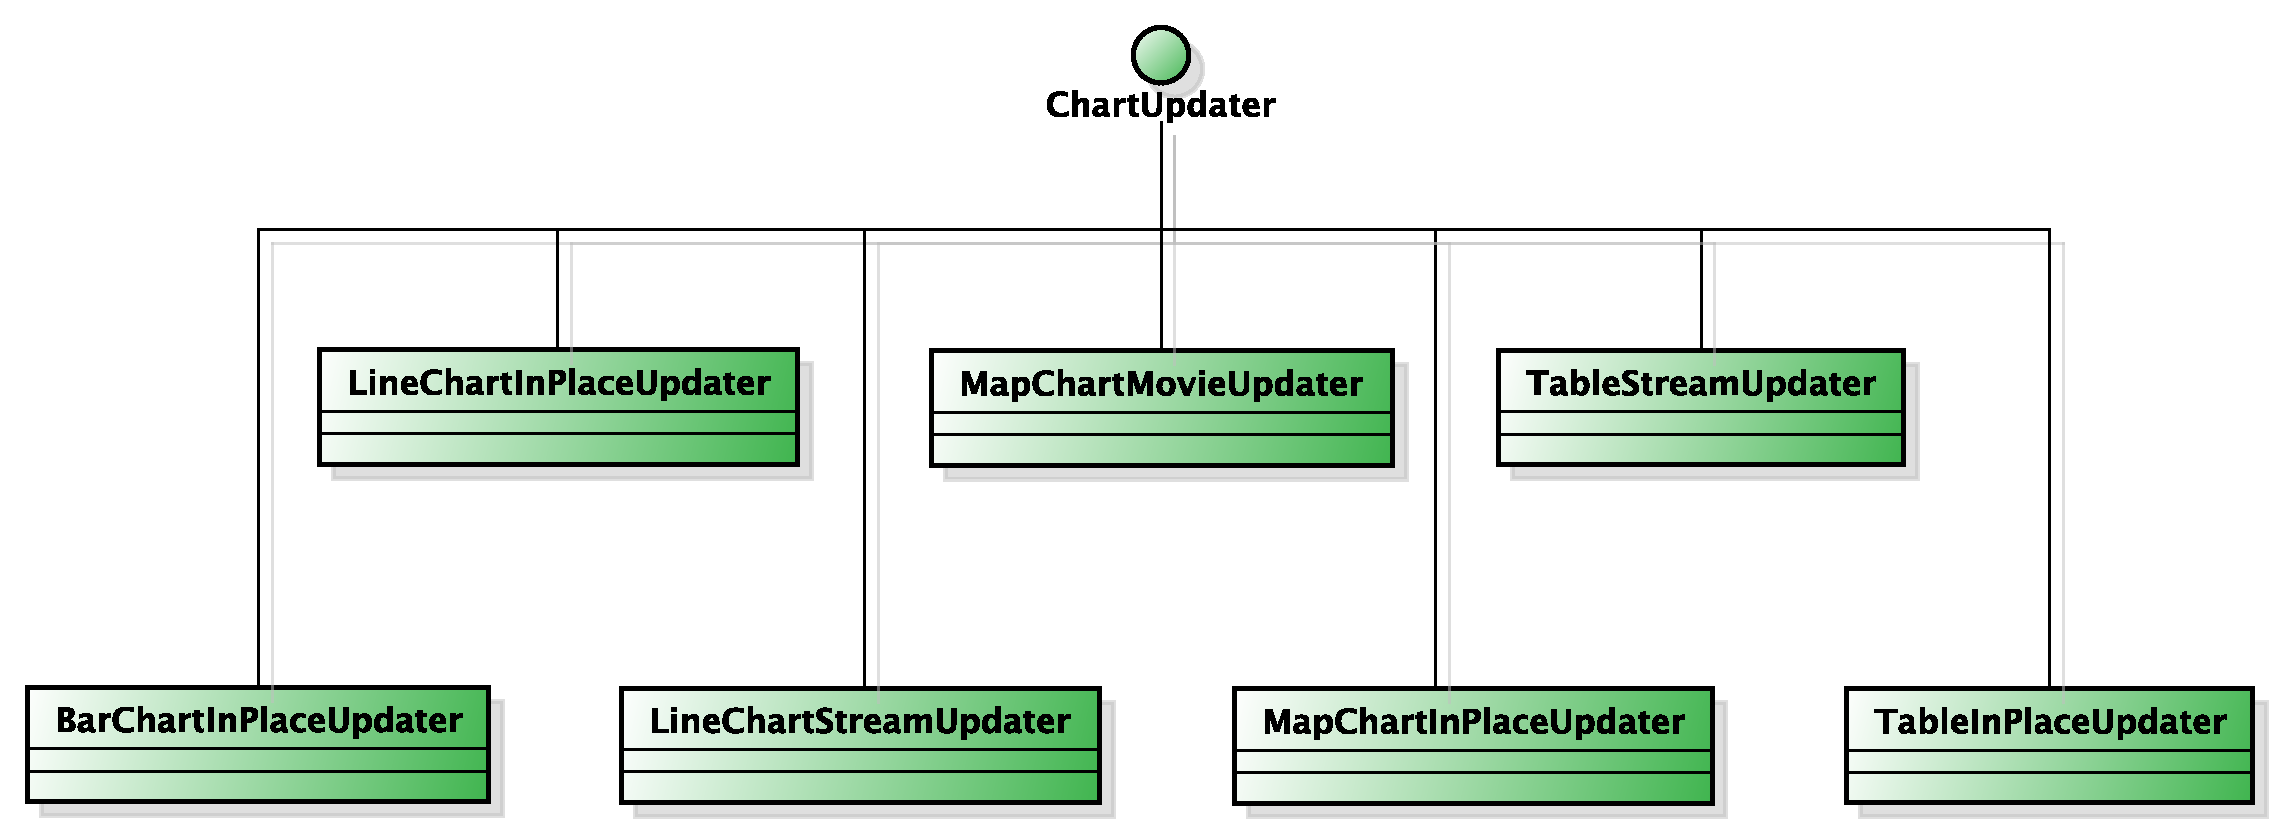
\includegraphics[width=1\textwidth]{DefinizioneDiProdotto/Pics/Gerarchie/ModelUpdater.pdf}
                        \caption{Diagramma gerarchia Updater in Chuck Model::NorrisChart }
                    \end{figure}
                \item Gerarchie in Model::Services \\
                    La seguente gerarchia rappresenta i servizi utilizzati in \insglo{Chuck}.
                    \begin{figure}[H]
                        \centering
                        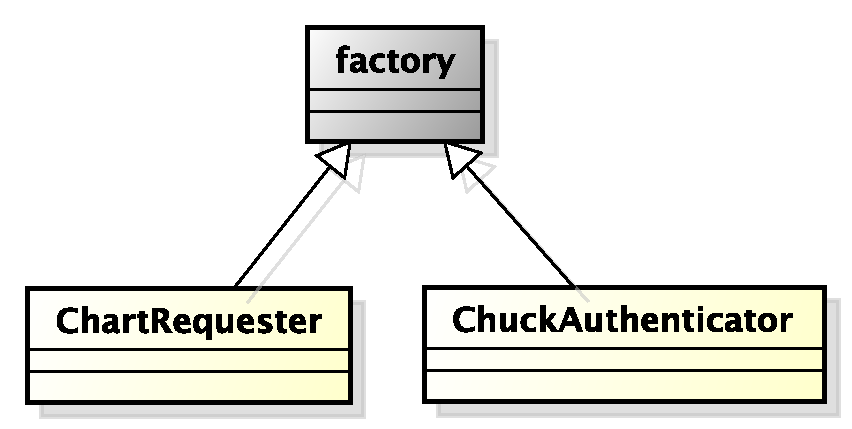
\includegraphics[width=1\textwidth]{DefinizioneDiProdotto/Pics/Gerarchie/ChuckService.pdf}
                        \caption{Diagramma gerarchia dei services in Chuck Model::Services}
                    \end{figure}
                \item Gerarchie in ViewModel \\
                    La seguente gerarchia rappresenta tutte le view-model utilizzate in \insglo{Chuck}.
                    \begin{figure}[H]
                        \centering
                        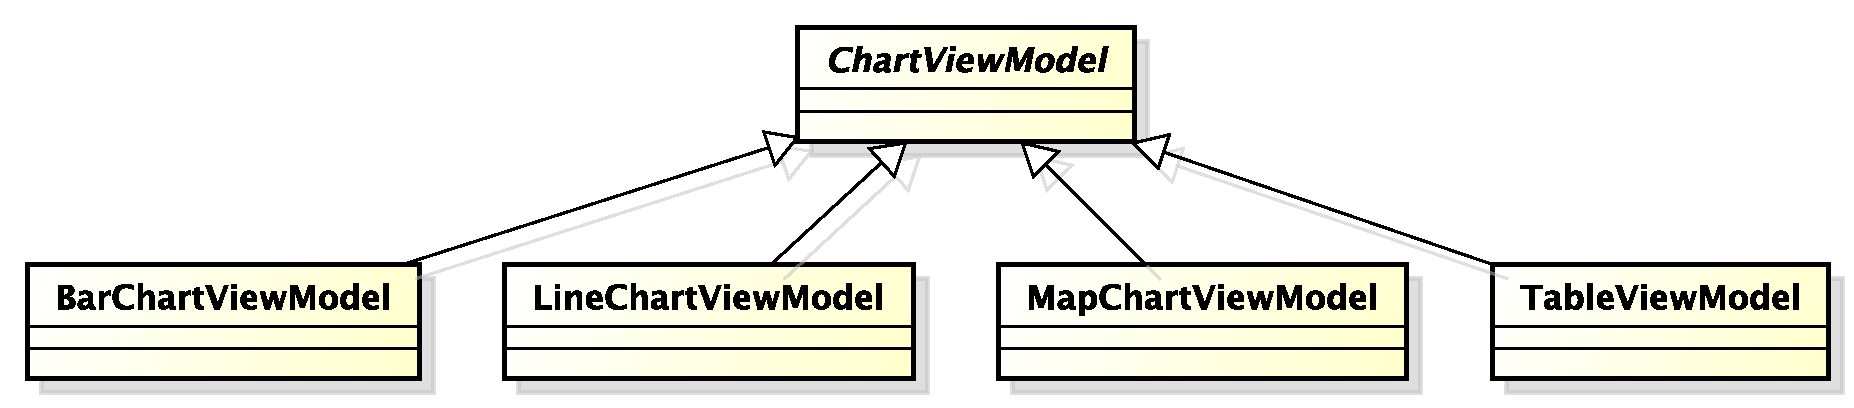
\includegraphics[width=1\textwidth]{DefinizioneDiProdotto/Pics/Gerarchie/ChuckViewModel.pdf}
                        \caption{Diagramma gerarchia dei view-model in Chuck ViewModel}
                    \end{figure}
                \item Gerarchie in Directive \\
                    La seguente gerarchia rappresenta le varie directive utilizzate in \insglo{Chuck}.
                    \begin{figure}[H]
                        \centering
                        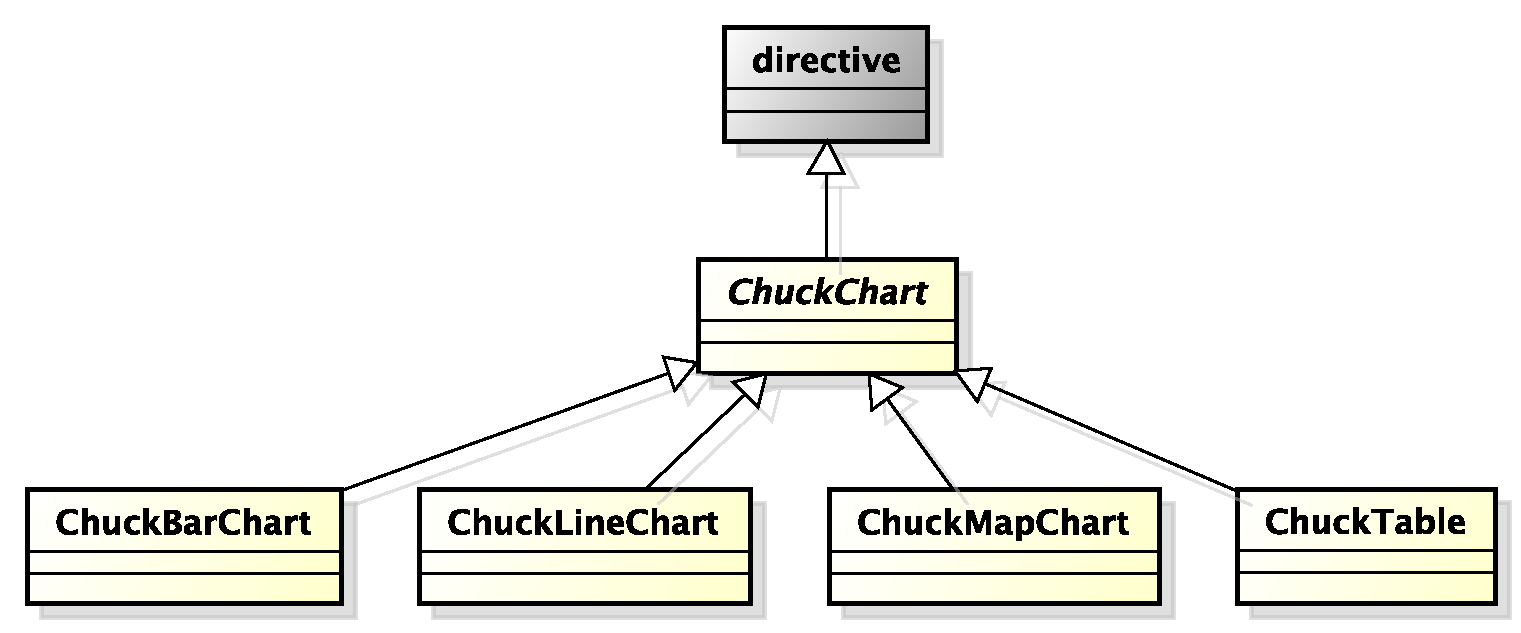
\includegraphics[width=1\textwidth]{DefinizioneDiProdotto/Pics/Gerarchie/ChuckDirective.pdf}
                        \caption{Diagramma gerarchia delle directive in Chuck Directive}
                    \end{figure}
                \item Gerarchie in View \\
                    La seguente gerarchia rappresenta le varie view utilizzate in \insglo{Chuck}.
                    \begin{figure}[H]
                        \centering
                        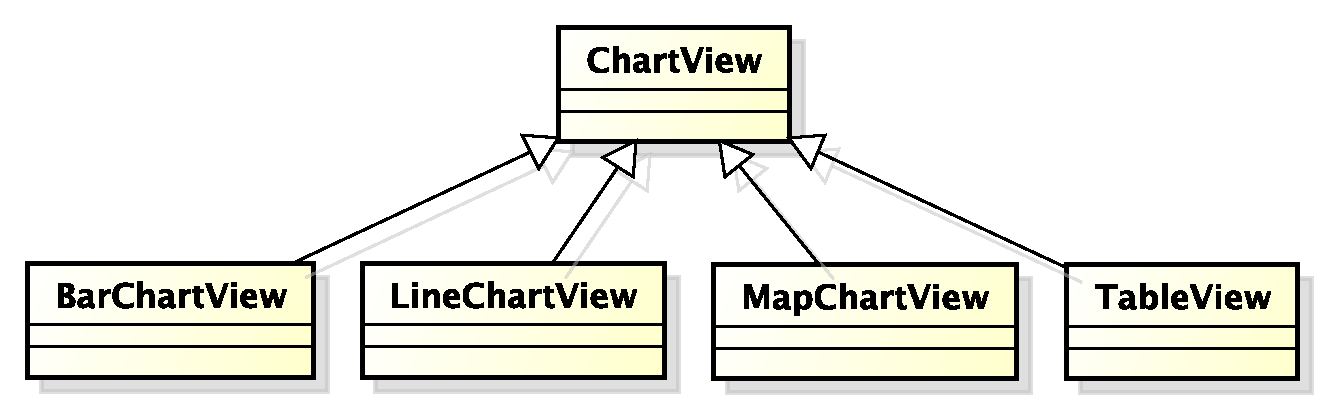
\includegraphics[width=1\textwidth]{DefinizioneDiProdotto/Pics/Gerarchie/ChuckView.pdf}
                        \caption{Diagramma gerarchia delle view in Chuck View}
                    \end{figure}
            \end{itemize}

        \level{3}{Classi}
            In tale sezione sono riportate delle descrizioni dettagliate delle classi individuate all'interno del documento \insdoc{Specifica Tecnica v4.00}. Tali classi sono presentate e organizzate in modo gerarchico, mantenendo una suddivisione per \insglo{package} di appartenenza.
            \input{Classi/Chuck.tex}

    \level{2}{Diagrammi di sequenza}
        In tale sezione vengono presentati i diagrammi di sequenza, che hanno lo scopo di descrivere scenari (determinate sequenze di azioni in cui tutte le scelte sono già state effettuate). Essi vengono usati per descrivere le relazioni che intercorrono, in termini di messaggi, tra attori, oggetti ed entità del sistema \insglo{Chuck}.
        \level{3}{Creazione di un chart}
             Tale diagramma riporta e descrive come viene creato un chart e collegato a quello presente all'interno di una certa istanza di \insglo{Norris}.
            \begin{figure}[H]
                \centering
                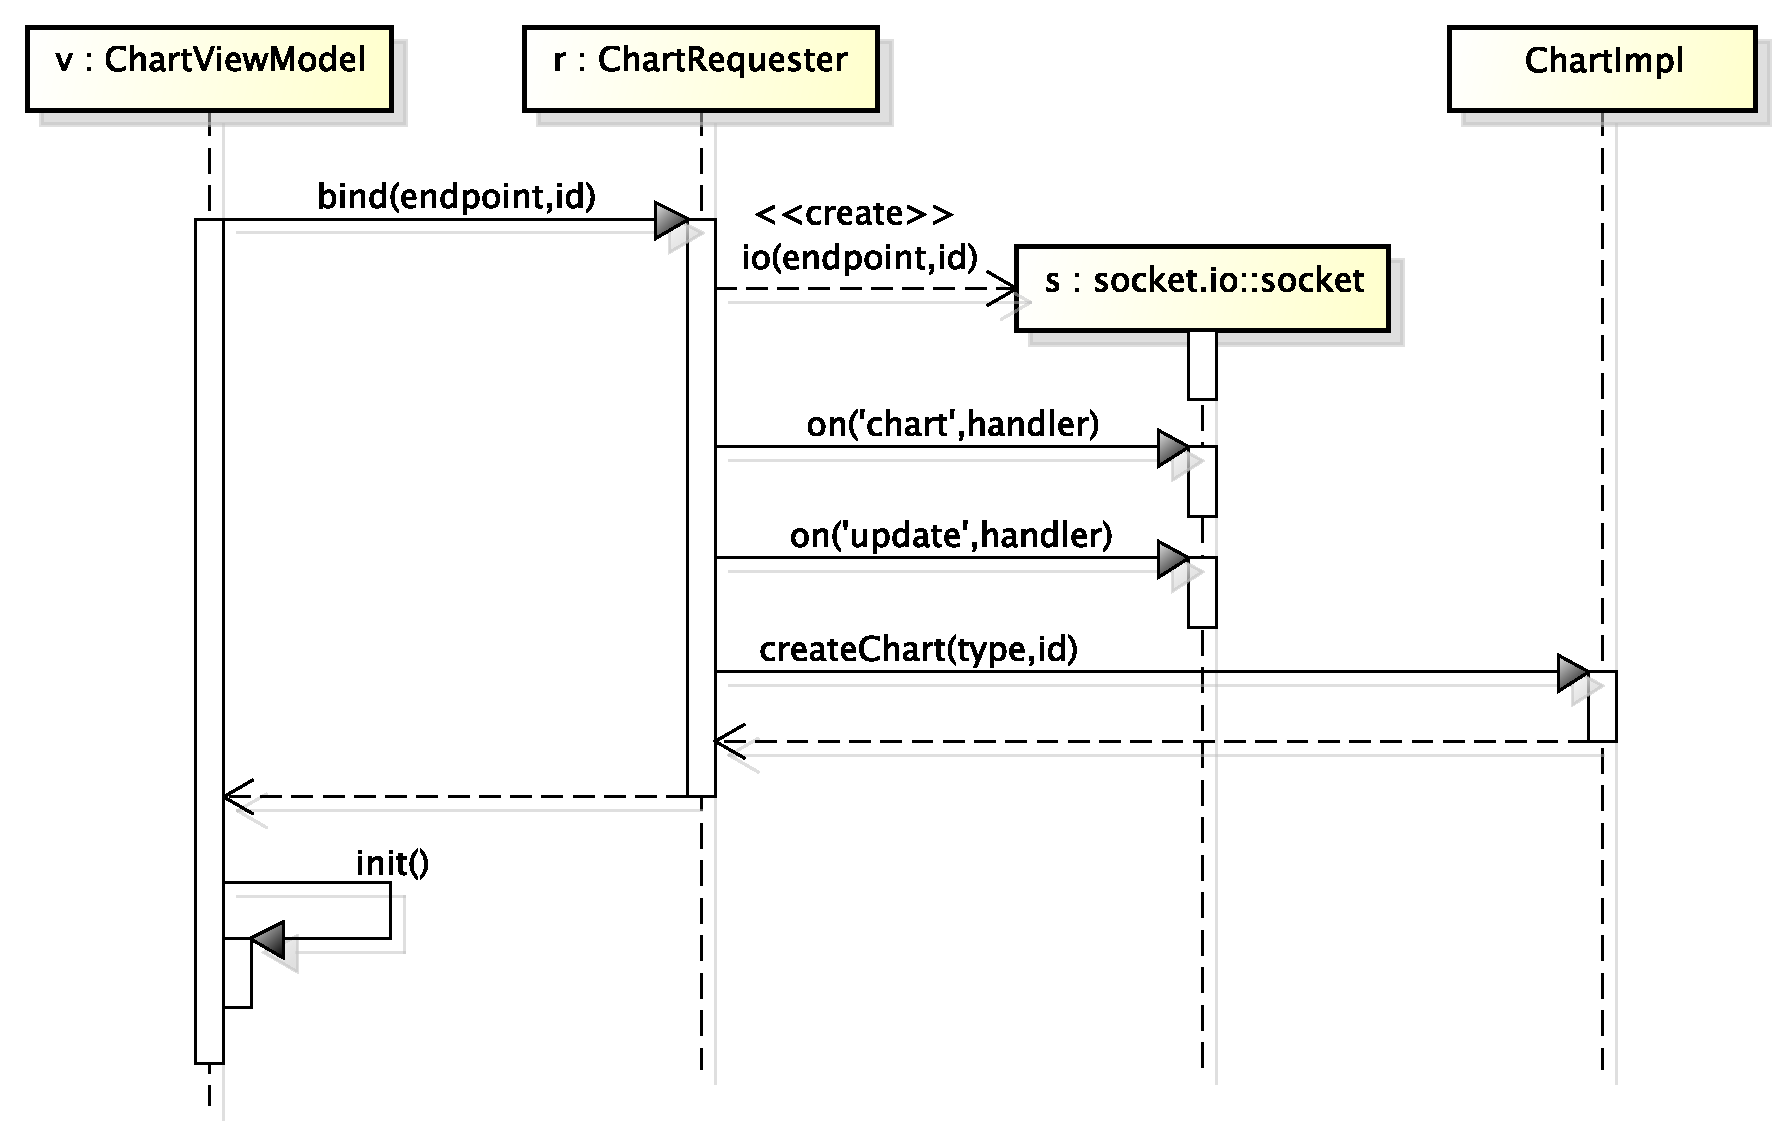
\includegraphics[scale=0.3]{DefinizioneDiProdotto/Pics/ChuckInserimentoChart}
                \caption{Diagramma di sequenza - Chuck, creazione chart}
            \end{figure}
            \begin{enumerate}
                \item ChartViewModel richiede l'ottenimento di un chart specifico presente in una istanza di \insglo{Norris} a ChartRequester;
                \item questo apre il canale socket ed imposta delle \insglo{callback} per gli eventi chart e update;
                \item ricevuto il grafico crea il modello dei dati;
                \item infine ChartViewModel esegue il metodo init che permette di inizializzare la view e visualizzare il Chart secondo i dati memorizzati.
            \end{enumerate}

        \level{3}{Aggiornamento di un chart}
            Tale diagramma descrive come viene aggiornato un chart nel momento in cui arrivano nuovi dati dall'istanza di \insglo{Norris} alla quale il grafico appartiene.
            \begin{figure}[H]
                \centering
                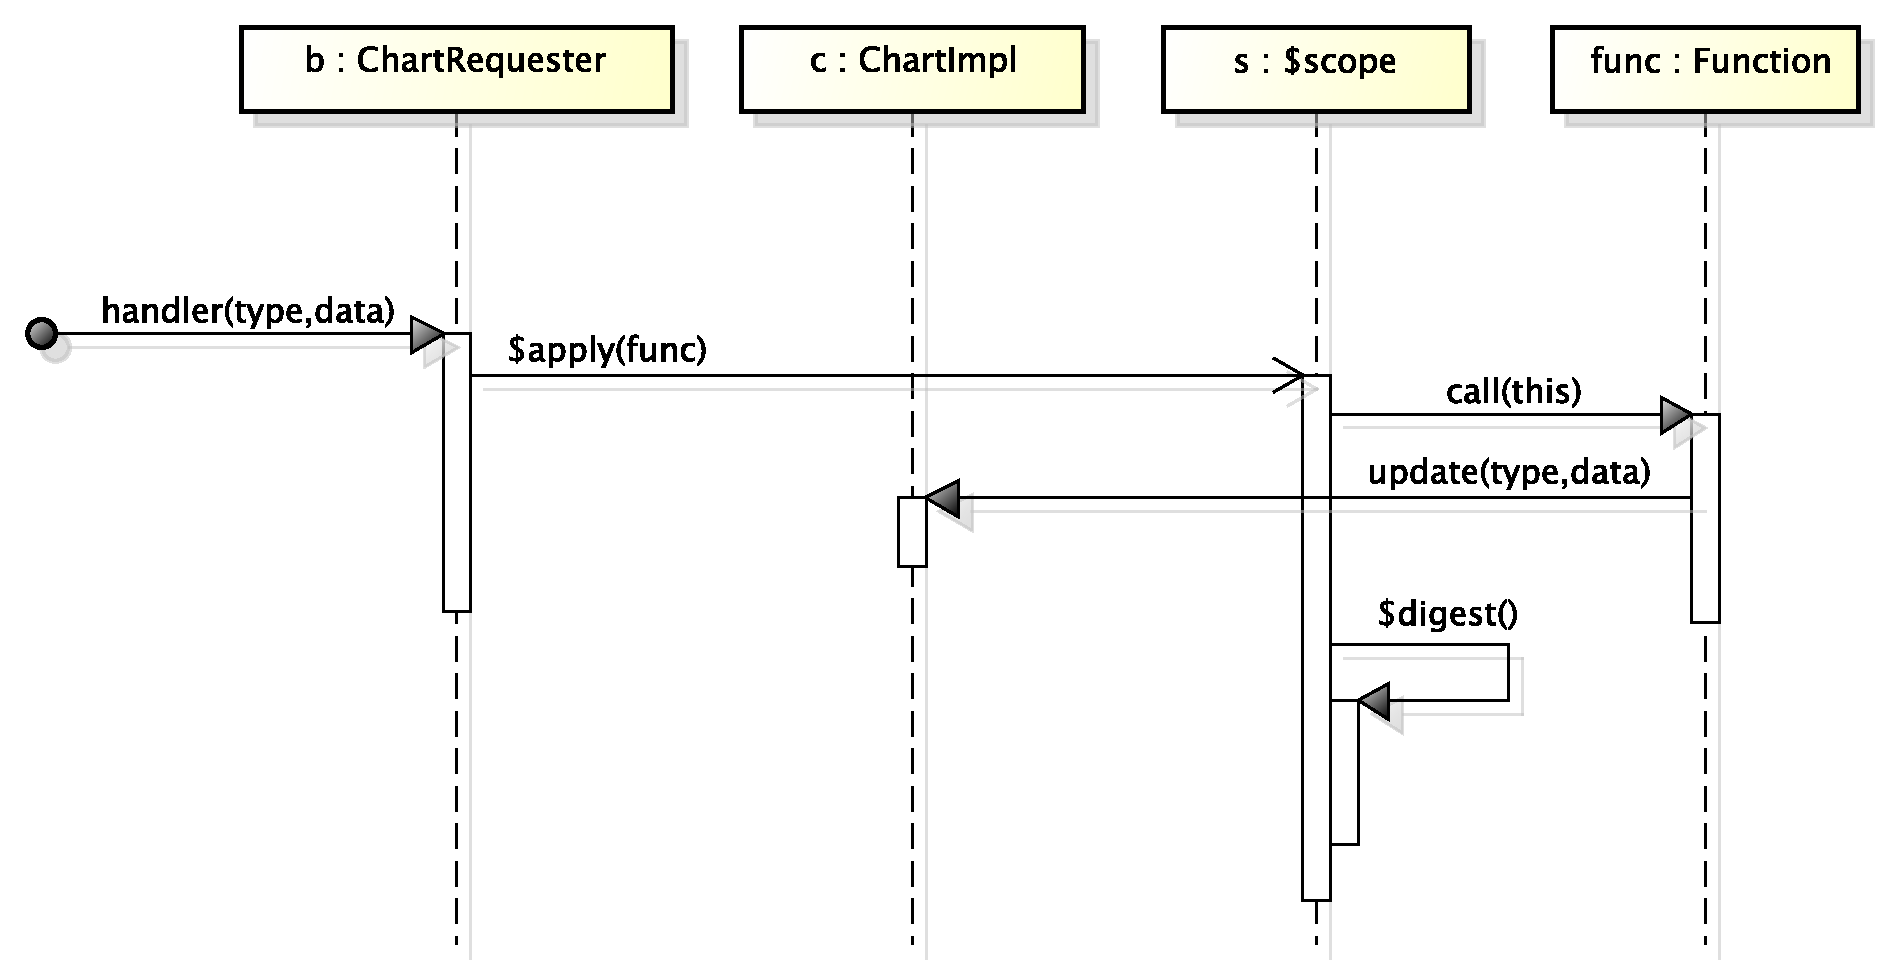
\includegraphics[scale=0.3]{DefinizioneDiProdotto/Pics/ChuckAggiornamentoChart}
                \caption{Diagramma di sequenza - Chuck, aggiornamento chart}
            \end{figure}
            \begin{enumerate}
                \item il messaggio iniziale rappresenta la notifica inviata da ChartRequester da parte di \insglo{Norris} attraverso il canale socket per avvertirlo dell'avvenuto aggiornamento;
                \item ChartRequester aggiorna il modello dei dati;
                \item avverte infine il ChartViewModel di un'avvenuta modifica nel modello richiedendo dunque la renderizzazione dei nuovi dati.
                \item
                \item
                \item
            \end{enumerate}


    \level{2}{Diagrammi di sequenza}
        In tale sezione vengono presentati i diagrammi di sequenza, che hanno lo scopo di descrivere scenari (determinate sequenze di azioni in cui tutte le scelte sono già state effettuate). Essi vengono usati per descrivere le relazioni che intercorrono, in termini di messaggi, tra attori, oggetti ed entità del sistema \insglo{Chuck}.
        \level{3}{Creazione di un chart}
             Tale diagramma riporta e descrive come viene creato un chart e collegato a quello presente all'interno di una certa istanza di \insglo{Norris}.
            \begin{figure}[H]
                \centering
                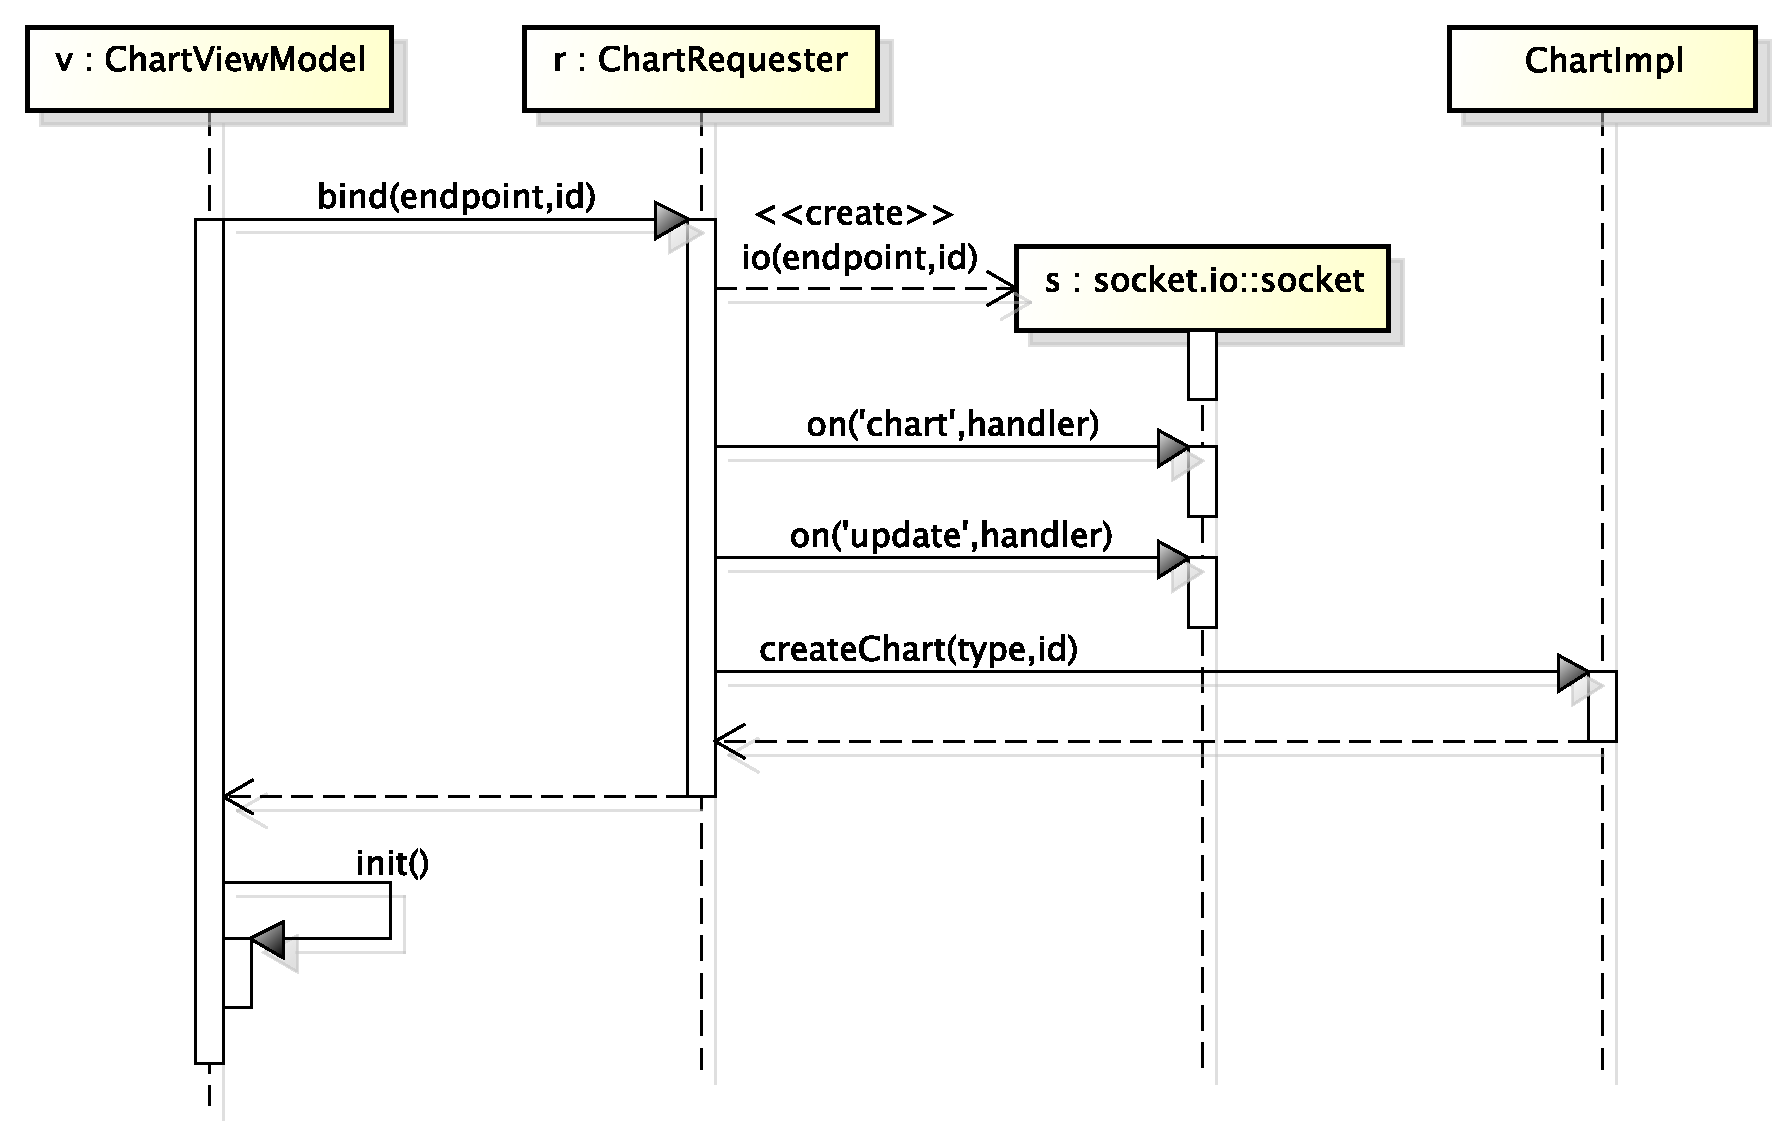
\includegraphics[scale=0.3]{DefinizioneDiProdotto/Pics/ChuckInserimentoChart}
                \caption{Diagramma di sequenza - Chuck, creazione chart}
            \end{figure}
            \begin{enumerate}
                \item ChartViewModel richiede l'ottenimento di un chart specifico presente in una istanza di \insglo{Norris} a ChartRequester;
                \item questo apre il canale socket ed imposta delle \insglo{callback} per gli eventi chart e update;
                \item ricevuto il grafico crea il modello dei dati;
                \item infine ChartViewModel esegue il metodo init che permette di inizializzare la view e visualizzare il Chart secondo i dati memorizzati.
            \end{enumerate}

        \level{3}{Aggiornamento di un chart}
            Tale diagramma descrive come viene aggiornato un chart nel momento in cui arrivano nuovi dati dall'istanza di \insglo{Norris} alla quale il grafico appartiene.
            \begin{figure}[H]
                \centering
                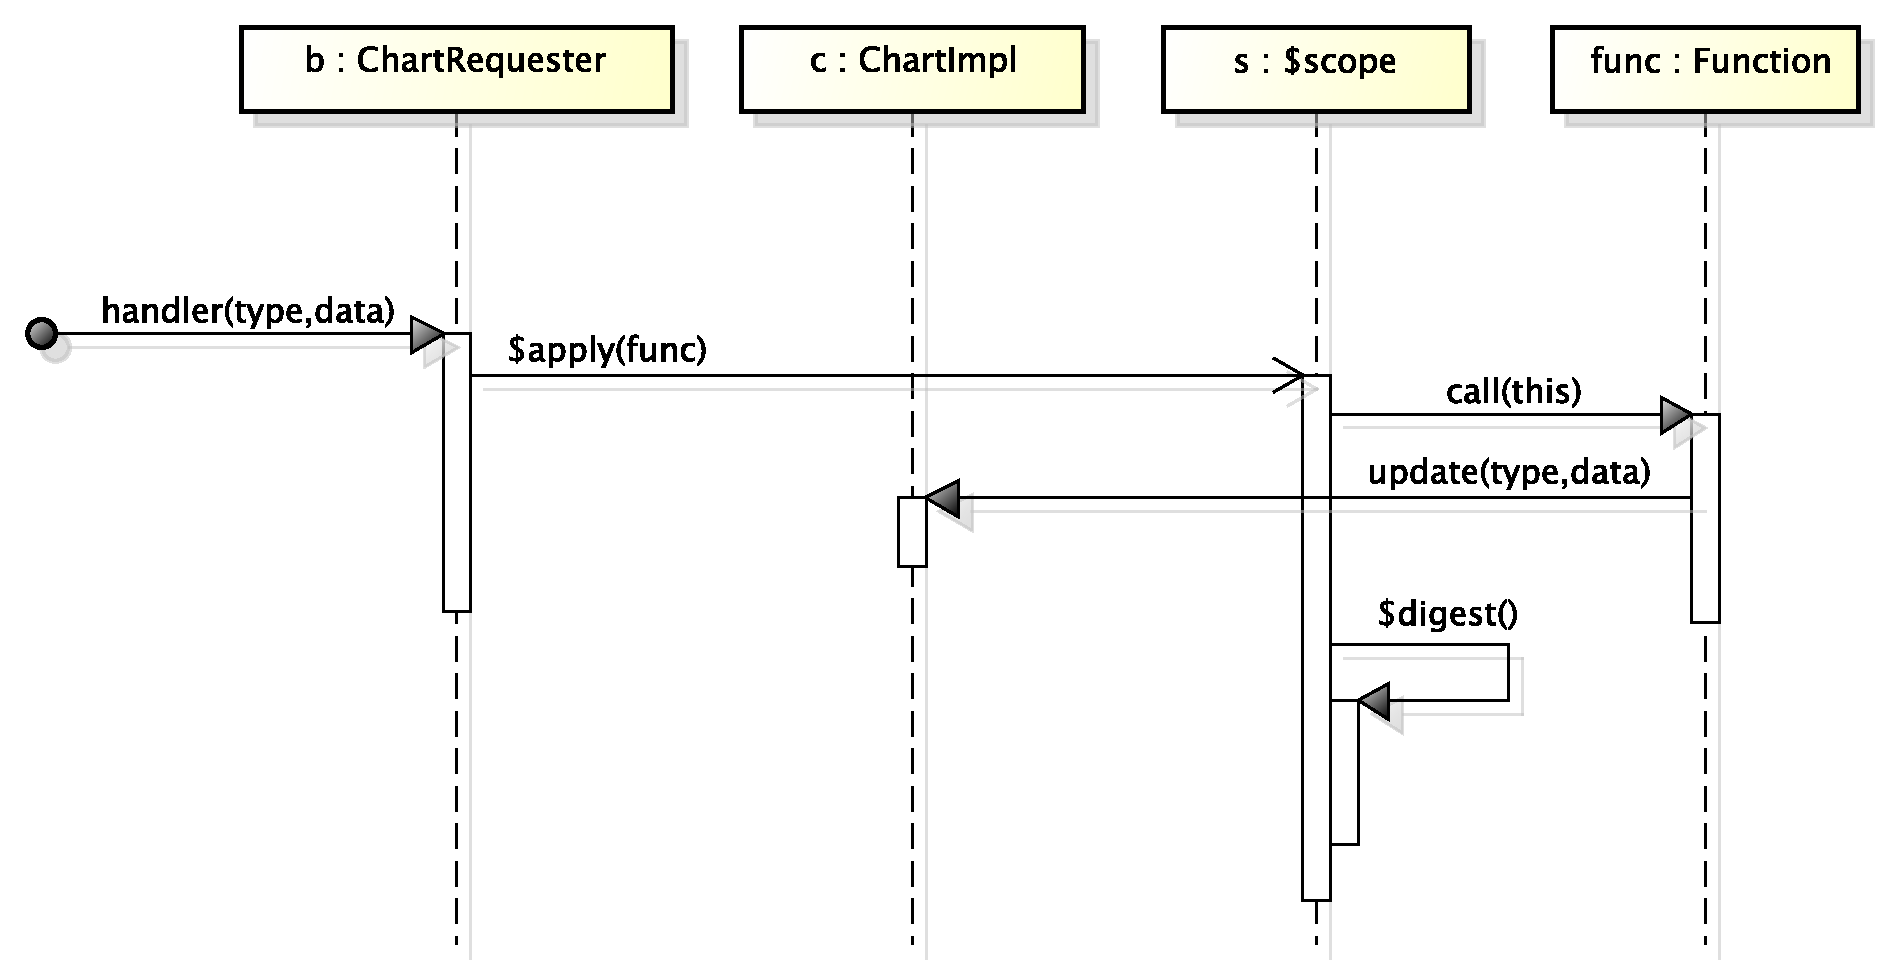
\includegraphics[scale=0.3]{DefinizioneDiProdotto/Pics/ChuckAggiornamentoChart}
                \caption{Diagramma di sequenza - Chuck, aggiornamento chart}
            \end{figure}
            \begin{enumerate}
                \item il messaggio iniziale rappresenta la notifica inviata da ChartRequester da parte di \insglo{Norris} attraverso il canale socket per avvertirlo dell'avvenuto aggiornamento;
                \item ChartRequester aggiorna il modello dei dati;
                \item avverte infine il ChartViewModel di un'avvenuta modifica nel modello richiedendo dunque la renderizzazione dei nuovi dati.
                \item
                \item
                \item
            \end{enumerate}


    \level{2}{Diagrammi di sequenza}
        In tale sezione vengono presentati i diagrammi di sequenza, che hanno lo scopo di descrivere scenari (determinate sequenze di azioni in cui tutte le scelte sono già state effettuate). Essi vengono usati per descrivere le relazioni che intercorrono, in termini di messaggi, tra attori, oggetti ed entità del sistema \insglo{Chuck}.
        \level{3}{Creazione di un chart}
             Tale diagramma riporta e descrive come viene creato un chart e collegato a quello presente all'interno di una certa istanza di \insglo{Norris}.
            \begin{figure}[H]
                \centering
                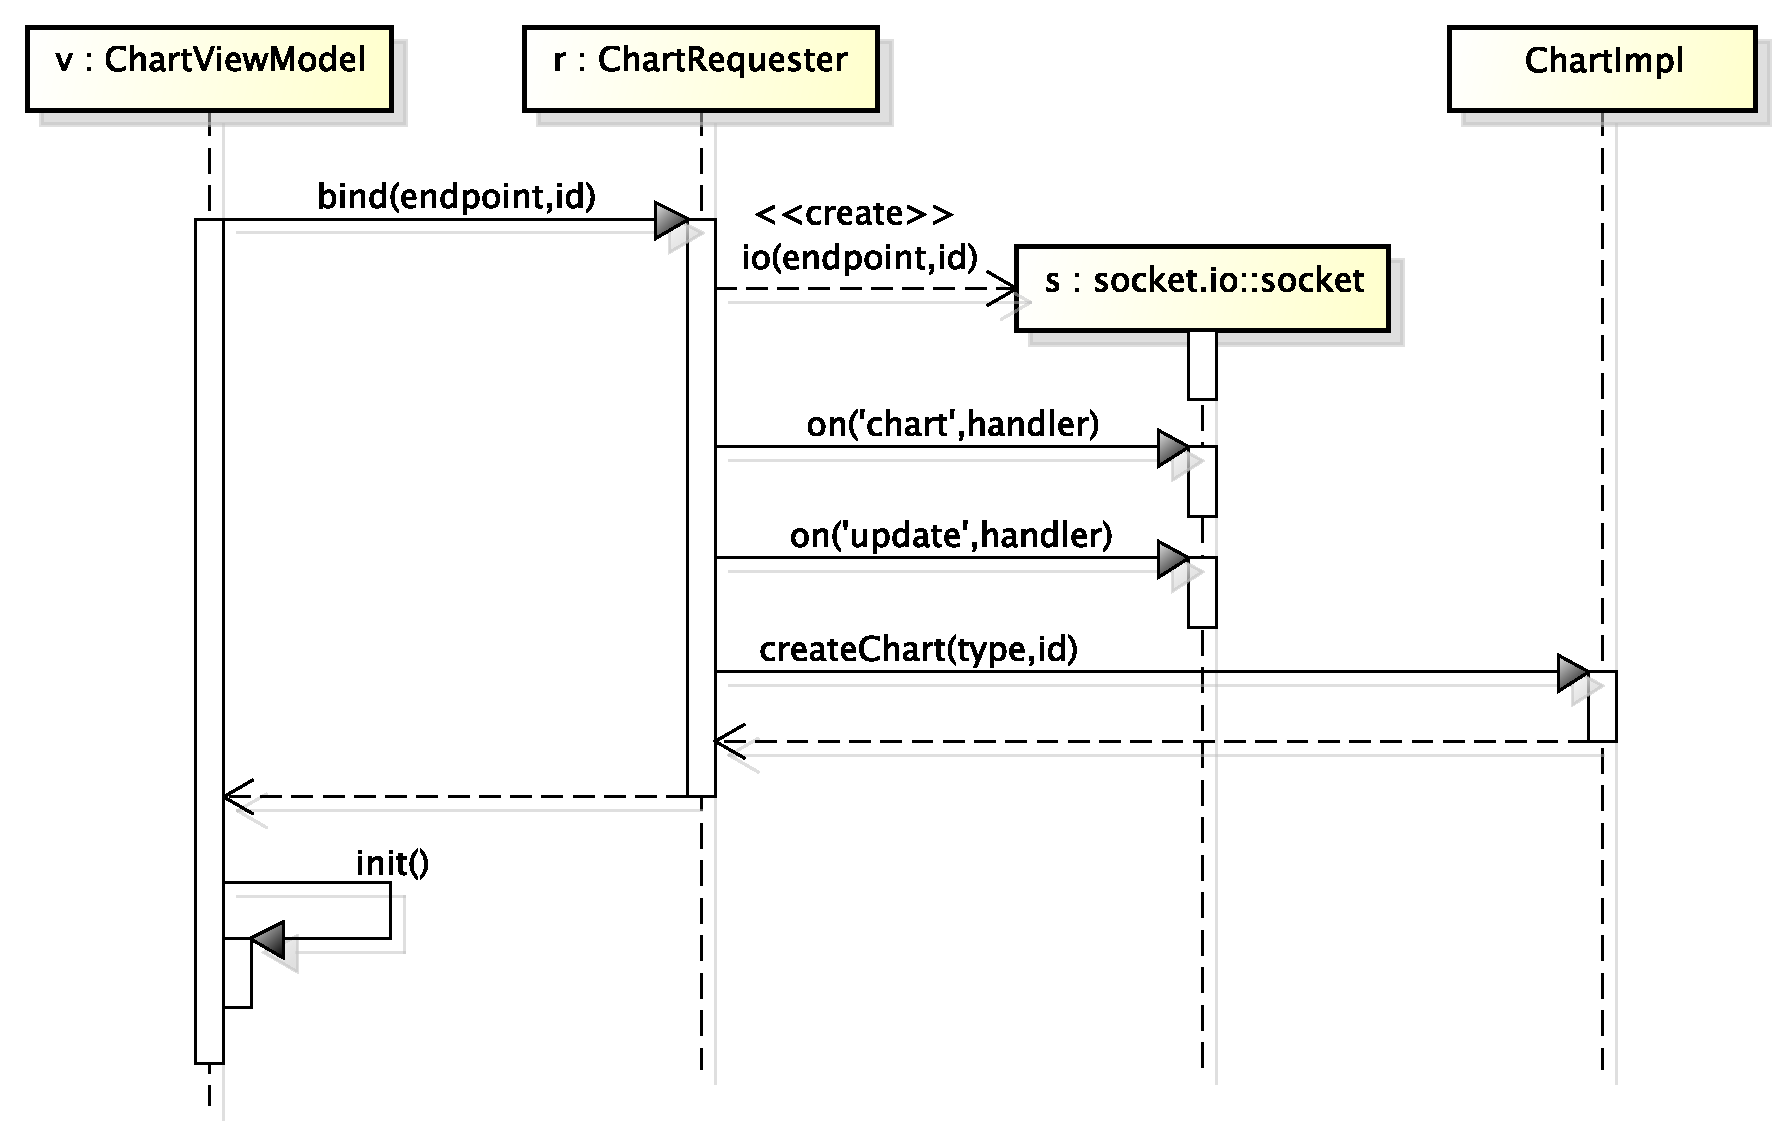
\includegraphics[scale=0.3]{DefinizioneDiProdotto/Pics/ChuckInserimentoChart}
                \caption{Diagramma di sequenza - Chuck, creazione chart}
            \end{figure}
            \begin{enumerate}
                \item ChartViewModel richiede l'ottenimento di un chart specifico presente in una istanza di \insglo{Norris} a ChartRequester;
                \item questo apre il canale socket ed imposta delle \insglo{callback} per gli eventi chart e update;
                \item ricevuto il grafico crea il modello dei dati;
                \item infine ChartViewModel esegue il metodo init che permette di inizializzare la view e visualizzare il Chart secondo i dati memorizzati.
            \end{enumerate}

        \level{3}{Aggiornamento di un chart}
            Tale diagramma descrive come viene aggiornato un chart nel momento in cui arrivano nuovi dati dall'istanza di \insglo{Norris} alla quale il grafico appartiene.
            \begin{figure}[H]
                \centering
                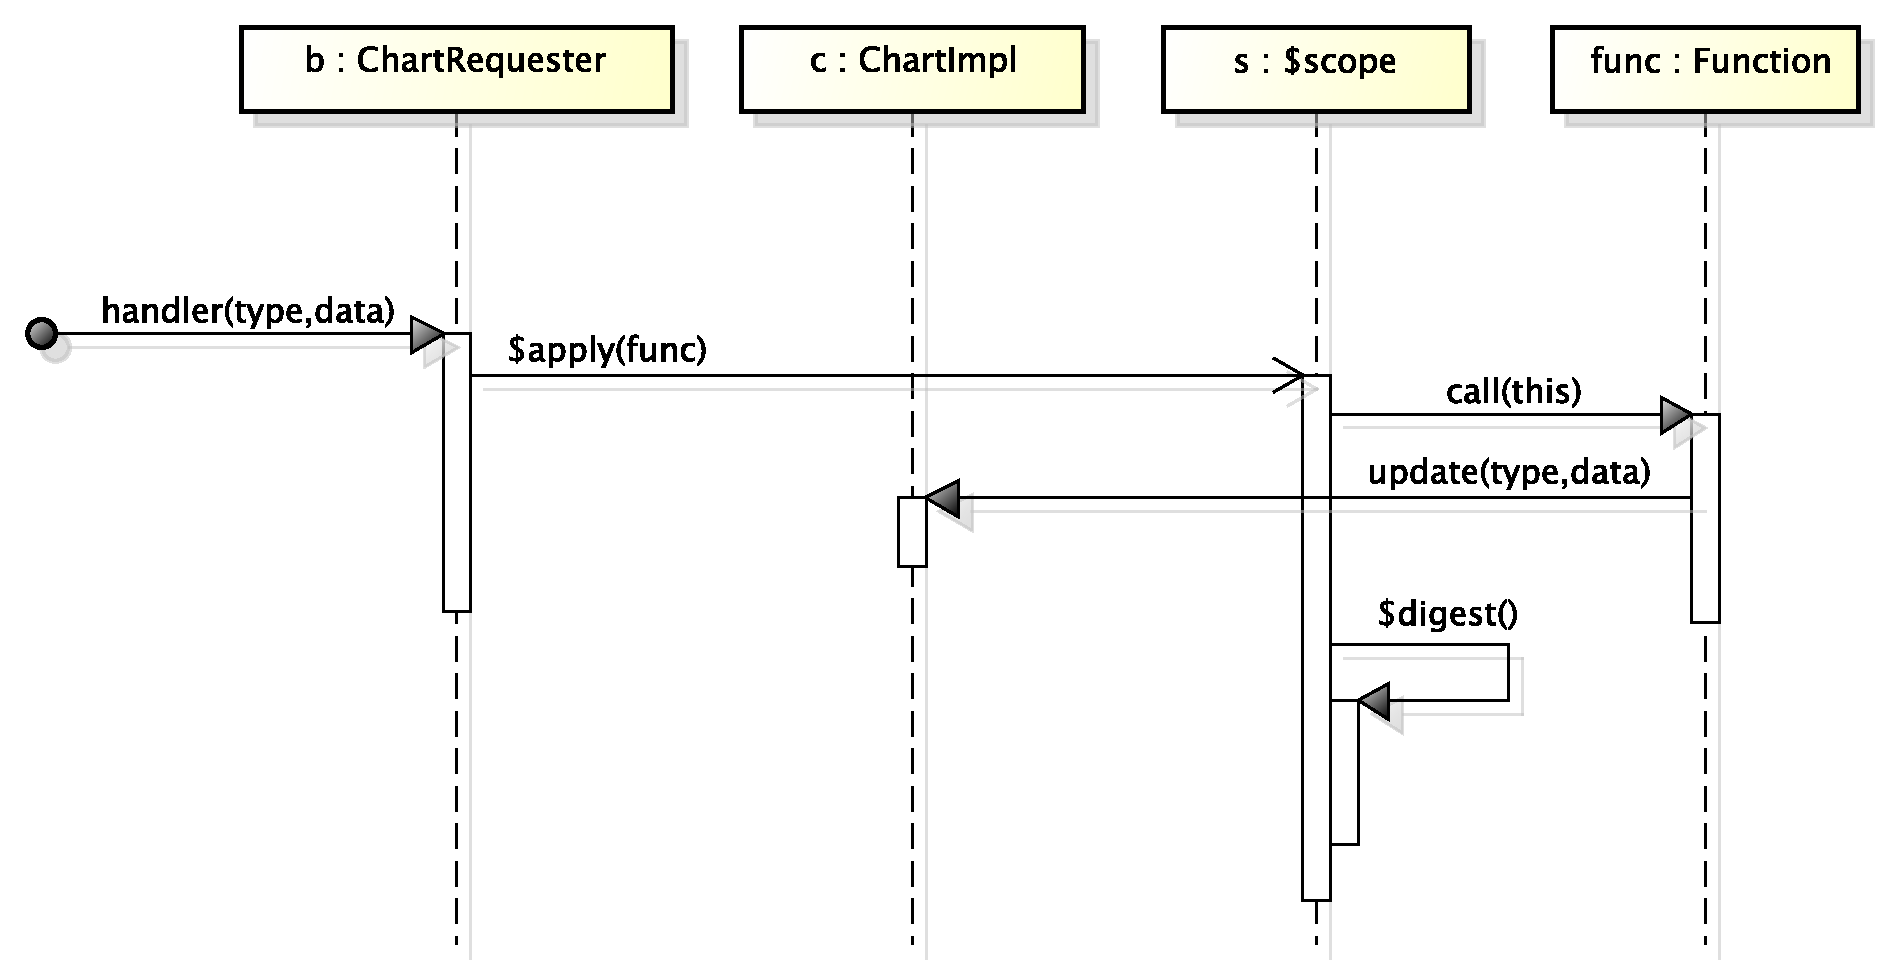
\includegraphics[scale=0.3]{DefinizioneDiProdotto/Pics/ChuckAggiornamentoChart}
                \caption{Diagramma di sequenza - Chuck, aggiornamento chart}
            \end{figure}
            \begin{enumerate}
                \item il messaggio iniziale rappresenta la notifica inviata da ChartRequester da parte di \insglo{Norris} attraverso il canale socket per avvertirlo dell'avvenuto aggiornamento;
                \item ChartRequester aggiorna il modello dei dati;
                \item avverte infine il ChartViewModel di un'avvenuta modifica nel modello richiedendo dunque la renderizzazione dei nuovi dati.
                \item
                \item
                \item
            \end{enumerate}

		\level{4}{Classi aggiuntive Chuck}
	Le interfacce \ignoreglo{Chuck::Model::NorrisChart::ChartData}, \ignoreglo{Chuck::Model::NorrisChart::ChartSettings} e \ignoreglo{Chuck::Model::NorrisChart::ChartUpdate} rappresentano genericamente i vari oggetti che utilizzeremo per rappresentare i dati, le impostazioni e gli aggiornamenti. Tali oggetti sono nel formato \insglo{JSON} ed essendo molto numerosi abbiamo deciso di non inserirle nel diagramma ma di elencarle e descriverle di seguito.

	\begin{itemize}
		\item \ignoreglo{\textbf{Chuck::Model::NorrisChart::BarChartData}} Questa classe implementa l'interfaccia \linebreak \insglo{Chuck}::Model::NorrisChart::ChartData. Essa si occupa di rappresentare i dati di un grafico \insglo{bar chart};

		\item \ignoreglo{\textbf{Chuck::Model::NorrisChart::LineChartData}} Questa classe implementa l'interfaccia \linebreak \insglo{Chuck}::Model::NorrisChart::ChartData. Essa si occupa di rappresentare i dati di un grafico \insglo{line chart};

		\item \ignoreglo{\textbf{Chuck::Model::NorrisChart::MapChartData}} Questa classe implementa l'interfaccia \linebreak \insglo{Chuck}::Model::NorrisChart::ChartData. Essa si occupa di rappresentare i dati di un grafico \insglo{map chart};

		\item \ignoreglo{\textbf{Chuck::Model::NorrisChart::TableData}} Questa classe implementa l'interfaccia \linebreak \insglo{Chuck}::Model::NorrisChart::ChartData. Essa si occupa di rappresentare i dati di un grafico \insglo{table};

		\item \ignoreglo{\textbf{Chuck::Model::NorrisChart::BarChartSetting}} Questa classe implementa l'interfaccia \linebreak \insglo{Chuck}::Model::NorrisChart::ChartSettings. Essa rappresenta le impostazioni di un grafico di tipo \insglo{bar chart};

		\item \ignoreglo{\textbf{Chuck::Model::NorrisChart::LineChartSetting}} Questa classe implementa l'interfaccia \linebreak \insglo{Chuck}::Model::NorrisChart::ChartSettings. Essa rappresenta le impostazioni di un grafico di tipo \insglo{line chart};

		\item \ignoreglo{\textbf{Chuck::Model::NorrisChart::MapChartSetting}} Questa classe implementa l'interfaccia \linebreak \insglo{Chuck}::Model::NorrisChart::ChartSettings. Essa rappresenta le impostazioni di un grafico di tipo \insglo{map chart};

		\item \ignoreglo{\textbf{Chuck::Model::NorrisChart::TableSetting}} Questa classe implementa l'interfaccia \linebreak \insglo{Chuck}::Model::NorrisChart::ChartSettings. Essa rappresenta le impostazioni di un grafico di tipo \insglo{table};

		\item \ignoreglo{\textbf{Chuck::Model::NorrisChart::BarChartInPlaceUpdate}} Questa classe implementa l'interfaccia \insglo{Chuck}::Model::NorrisChart::ChartUpdate. Essa rappresenta un pacchetto di aggiornamento di tipo \insglo{in place} per un grafico di tipo \insglo{bar chart};

		\item \ignoreglo{\textbf{Chuck::Model::NorrisChart::LineChartInPlaceUpdate}} Questa classe implementa l'interfaccia \insglo{Chuck}::Model::NorrisChart::ChartUpdate. Essa rappresenta un pacchetto di aggiornamento di tipo \insglo{in place} per un grafico di tipo \insglo{line chart};

		\item \ignoreglo{\textbf{Chuck::Model::NorrisChart::LineChartStreamUpdate}} Questa classe implementa l'interfaccia \insglo{Chuck}::Model::NorrisChart::ChartUpdate. Essa rappresenta un pacchetto di aggiornamento di tipo \insglo{stream} per un grafico di tipo \insglo{line chart};

		\item \ignoreglo{\textbf{Chuck::Model::NorrisChart::MapChartInPlaceUpdate}} Questa classe implementa l'interfaccia \insglo{Chuck}::Model::NorrisChart::ChartUpdate. Essa rappresenta un pacchetto di aggiornamento di tipo \insglo{in place} per un grafico di tipo \insglo{map chart};

		\item \ignoreglo{\textbf{Chuck::Model::NorrisChart::MapChartMovieUpdate}} Questa classe implementa l'interfaccia \insglo{Chuck}::Model::NorrisChart::ChartUpdate. Essa rappresenta un pacchetto di aggiornamento di tipo \insglo{movie} per un grafico di tipo \insglo{map chart};

		\item \ignoreglo{\textbf{Chuck::Model::NorrisChart::TableStreamUpdate}} Questa classe implementa l'interfaccia \insglo{Chuck}::Model::NorrisChart::ChartUpdate. Essa rappresenta un pacchetto di aggiornamento di tipo \insglo{stream} per un grafico di tipo \insglo{table};

		\item \ignoreglo{\textbf{Chuck::Model::NorrisChart::TableInPlaceUpdate}} Questa classe implementa l'interfaccia \insglo{Chuck}::Model::NorrisChart::ChartUpdate. Essa rappresenta un pacchetto di aggiornamento di tipo \insglo{in place} per un grafico di tipo \insglo{table}.
	\end{itemize}

	\level{2}{Interazioni tra classi dei componenti di Chuck}
	Dopo che sono stati descritte nel dettaglio tutte le varie classi necessarie alla progettazione di \insglo{Chuck}, è necessario mostrare come le classi appartenenti a componenti differenti interagiscano tra di loro. È quindi inserito in seguito un diagramma \insglo{UML} che rappresenta tutte le interazioni presenti tra i vari componenti.\\
	Si noti che alcune classi non sono state inserite in quanto si è voluto rendere più comprensibile il diagramma.

	\begin{figure}[H]\centering
		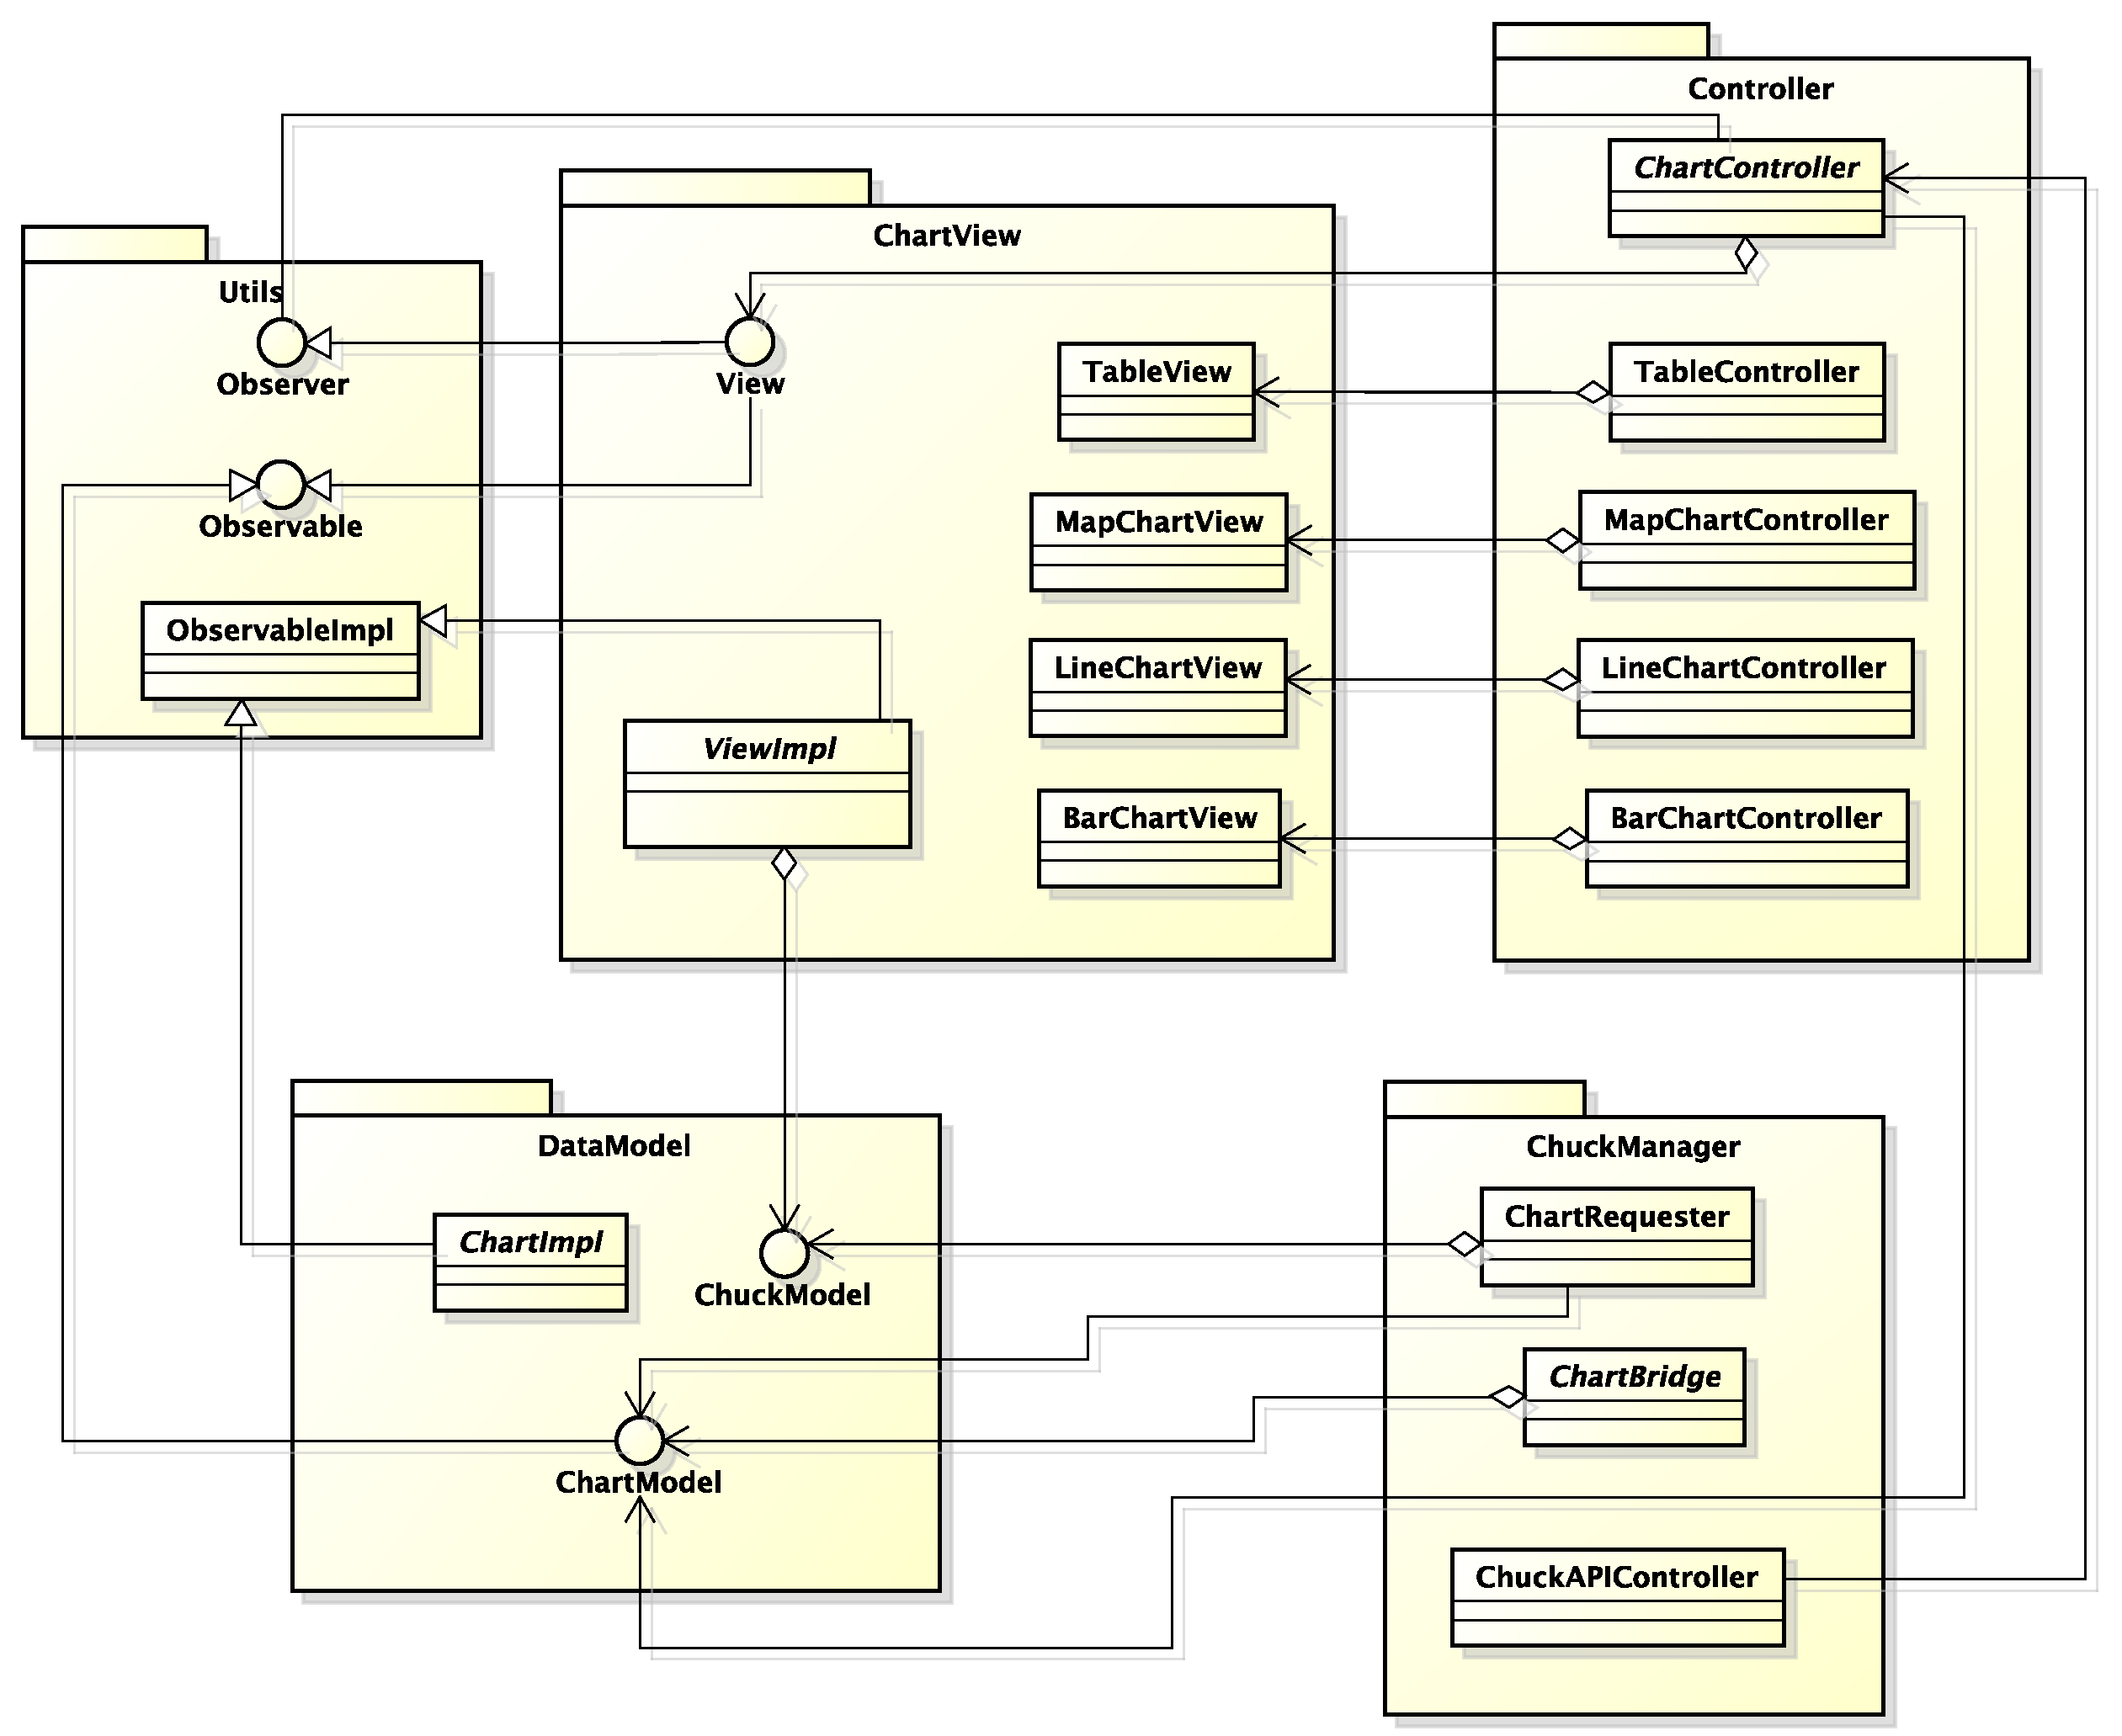
\includegraphics[width=\textwidth]{SpecificaTecnica/Pics/InterazioniComponentiChuck.pdf}
		\caption{Diagramma delle interazioni tra classi di componenti di Chuck}
	\end{figure}
	\level{3}{Design pattern utilizzati con le classi}
		Nella progettazione delle classi di \insglo{Chuck} abbiamo deciso di utilizzare alcuni \insglo{design pattern}. Riportiamo di seguito una loro breve descrizione e il contesto nel quale sono stati utilizzati.
		\level{4}{Bridge}
			Il Bridge è un \insglo{pattern} strutturale pensato per separare l'interfaccia di una classe dalla sua implementazione. In particolare, utilizza i concetti di \textit{encapsulation}, \textit{aggregation} ed \textit{inheritance} per separare varie responsabilità in classi differenti. \\
			Il \insglo{design pattern} Bridge si differenzia dal \insglo{pattern} Adapter, in quanto il primo viene utilizzato fin dall'inizio della progettazione per consentire ad astrazioni ed implementazioni di variare in modo indipendente, mentre il secondo viene usato quando si vogliono adattare classi inizialmente non correlate e viene introdotto dopo che queste sono state progettate.
			Per una descrizione più approfondita del \insglo{pattern} e dei vantaggi derivanti dalla sua applicazione si rimanda all'appendice \nameref{app:bridge}.
			\level{5}{Contesto di utilizzo}
				In \insglo{Chuck} questo \insglo{pattern} viene utilizzato nel \insglo{package} ChuckAPIManager per separare l'implementazione dei chart (presente nel \insglo{package} DataModel) dall'interfaccia fornita allo sviluppatore \insglo{client}.
		\level{4}{Dependency Injection}
			Dependency Injection è un \insglo{pattern} architetturale il cui scopo è separare il comportamento di una componente dalla risoluzione delle sue dipendenze.\\
			Per la descrizione del \insglo{pattern} e dei vantaggi derivanti dalla sua applicazione si rimanda all'appendice \nameref{app:dependencyinjection}.
			\level{5}{Contesto di utilizzo}
				La Dependency Injection viene utilizzata con le classi che implementano le interfaccie DataModel::ChartFactory e DataModel::Updater. Attraverso queste classi vengono "iniettate" nella classe DataModel::ChartImpl rispettivamente le corrispondenze tra i tipi di grafico e le rispettive classi factory e le corrispondenze tra i diversi tipi di aggiornamenti e le classi che li implementano.
		\level{4}{Singleton}
			Il Singleton è un \insglo{pattern} creazionale il cui scopo è permettere la creazione di una sola istanza di una classe e fornire un punto di accesso globale ad essa.\\
			Per la descrizione del \insglo{pattern} e dei vantaggi derivanti dalla sua applicazione si rimanda all'appendice \nameref{app:singleton}.
			\level{5}{Contesto di utilizzo}
				Le classi che implementano il Singleton sono quelle che si occupano di creare i diversi tipi di grafici. cioè:
				\begin{itemize}
					\item DataModel::BarChartFactory;
					\item DataModel::LineChartFactory;
					\item DataModel::MapChartFactory;
					\item DataModel::TableFactory.
			\end{itemize}
		\level{4}{Abstract Factory}
			Il \insglo{pattern} creazionale Abstract Factory si occupa di fornire un'interfaccia per la creazione di famiglie di prodotti, senza dover specificare classi concrete. \\
			Per la descrizione del \insglo{pattern} e dei vantaggi derivanti dalla sua applicazione si rimanda all'appendice \nameref{app:abstractfactory}.
			\level{5}{Contesto di utilizzo}
				Gli elementi che implementano Abstract Factory sono:
				\begin{itemize}
				\item Interfacce:
					\begin{itemize}
						\item DataModel::ChartFactory, con cui vengono generati i diversi tipi di grafici.
					\end{itemize}
				\item Classi:
					\begin{itemize}
						\item DataModel::BarChartFactory;
						\item DataModel::LineChartFactory;
						\item DataModel::MapChartFactory;
						\item DataModel::TableFactory.
					\end{itemize}
				\end{itemize}
		\level{4}{Adapter}
			Il \insglo{pattern} strutturale Adapter viene utilizzato per adattare l'interfaccia di una classe in un'altra.\\
			Per la descrizione del \insglo{pattern} e dei vantaggi derivanti dalla sua applicazione si rimanda all'appendice \nameref{app:adapter}.
			\level{5}{Contesto di utilizzo}
				In \insglo{Chuck} l'Adapter viene utilizzato per calare le varie librerie esterne nel contesto di \projectname{}, e nello specifico sono rappresentate dalle diverse View, quindi:
				\begin{itemize}
					\item View::BarChartView e View::LineChartView sono adattatori per \insglo{Chart.js};
					\item View::MapChartView è un adattatore per OpenStreetMaps;
					\item View::TableView è un adattatore per Dynatable.
				\end{itemize}